% !TeX root = ../main.tex

\appendix{A}{結果與評估}
\section{結果}

{\footnotesize
\renewcommand{\arraystretch}{0.8}
\begin{longtable}{
  >{\centering\arraybackslash}m{1cm}
  >{\centering\arraybackslash}m{5cm}
  >{\arraybackslash}m{2cm}
  >{\arraybackslash}m{2cm}
  >{\arraybackslash}m{3cm}
}
\caption{研究結果} \label{tab:results} \\
\toprule
項次 & 圖面／經緯度坐標 & 本研究機制 & 人工撰寫 & GPT-4o \\
\midrule
\endfirsthead

\midrule
項次 & 圖面／經緯度坐標 & 本研究機制 & 人工撰寫 & GPT-4o \\
\midrule
\endhead
\bottomrule
\endlastfoot
1-1 & 
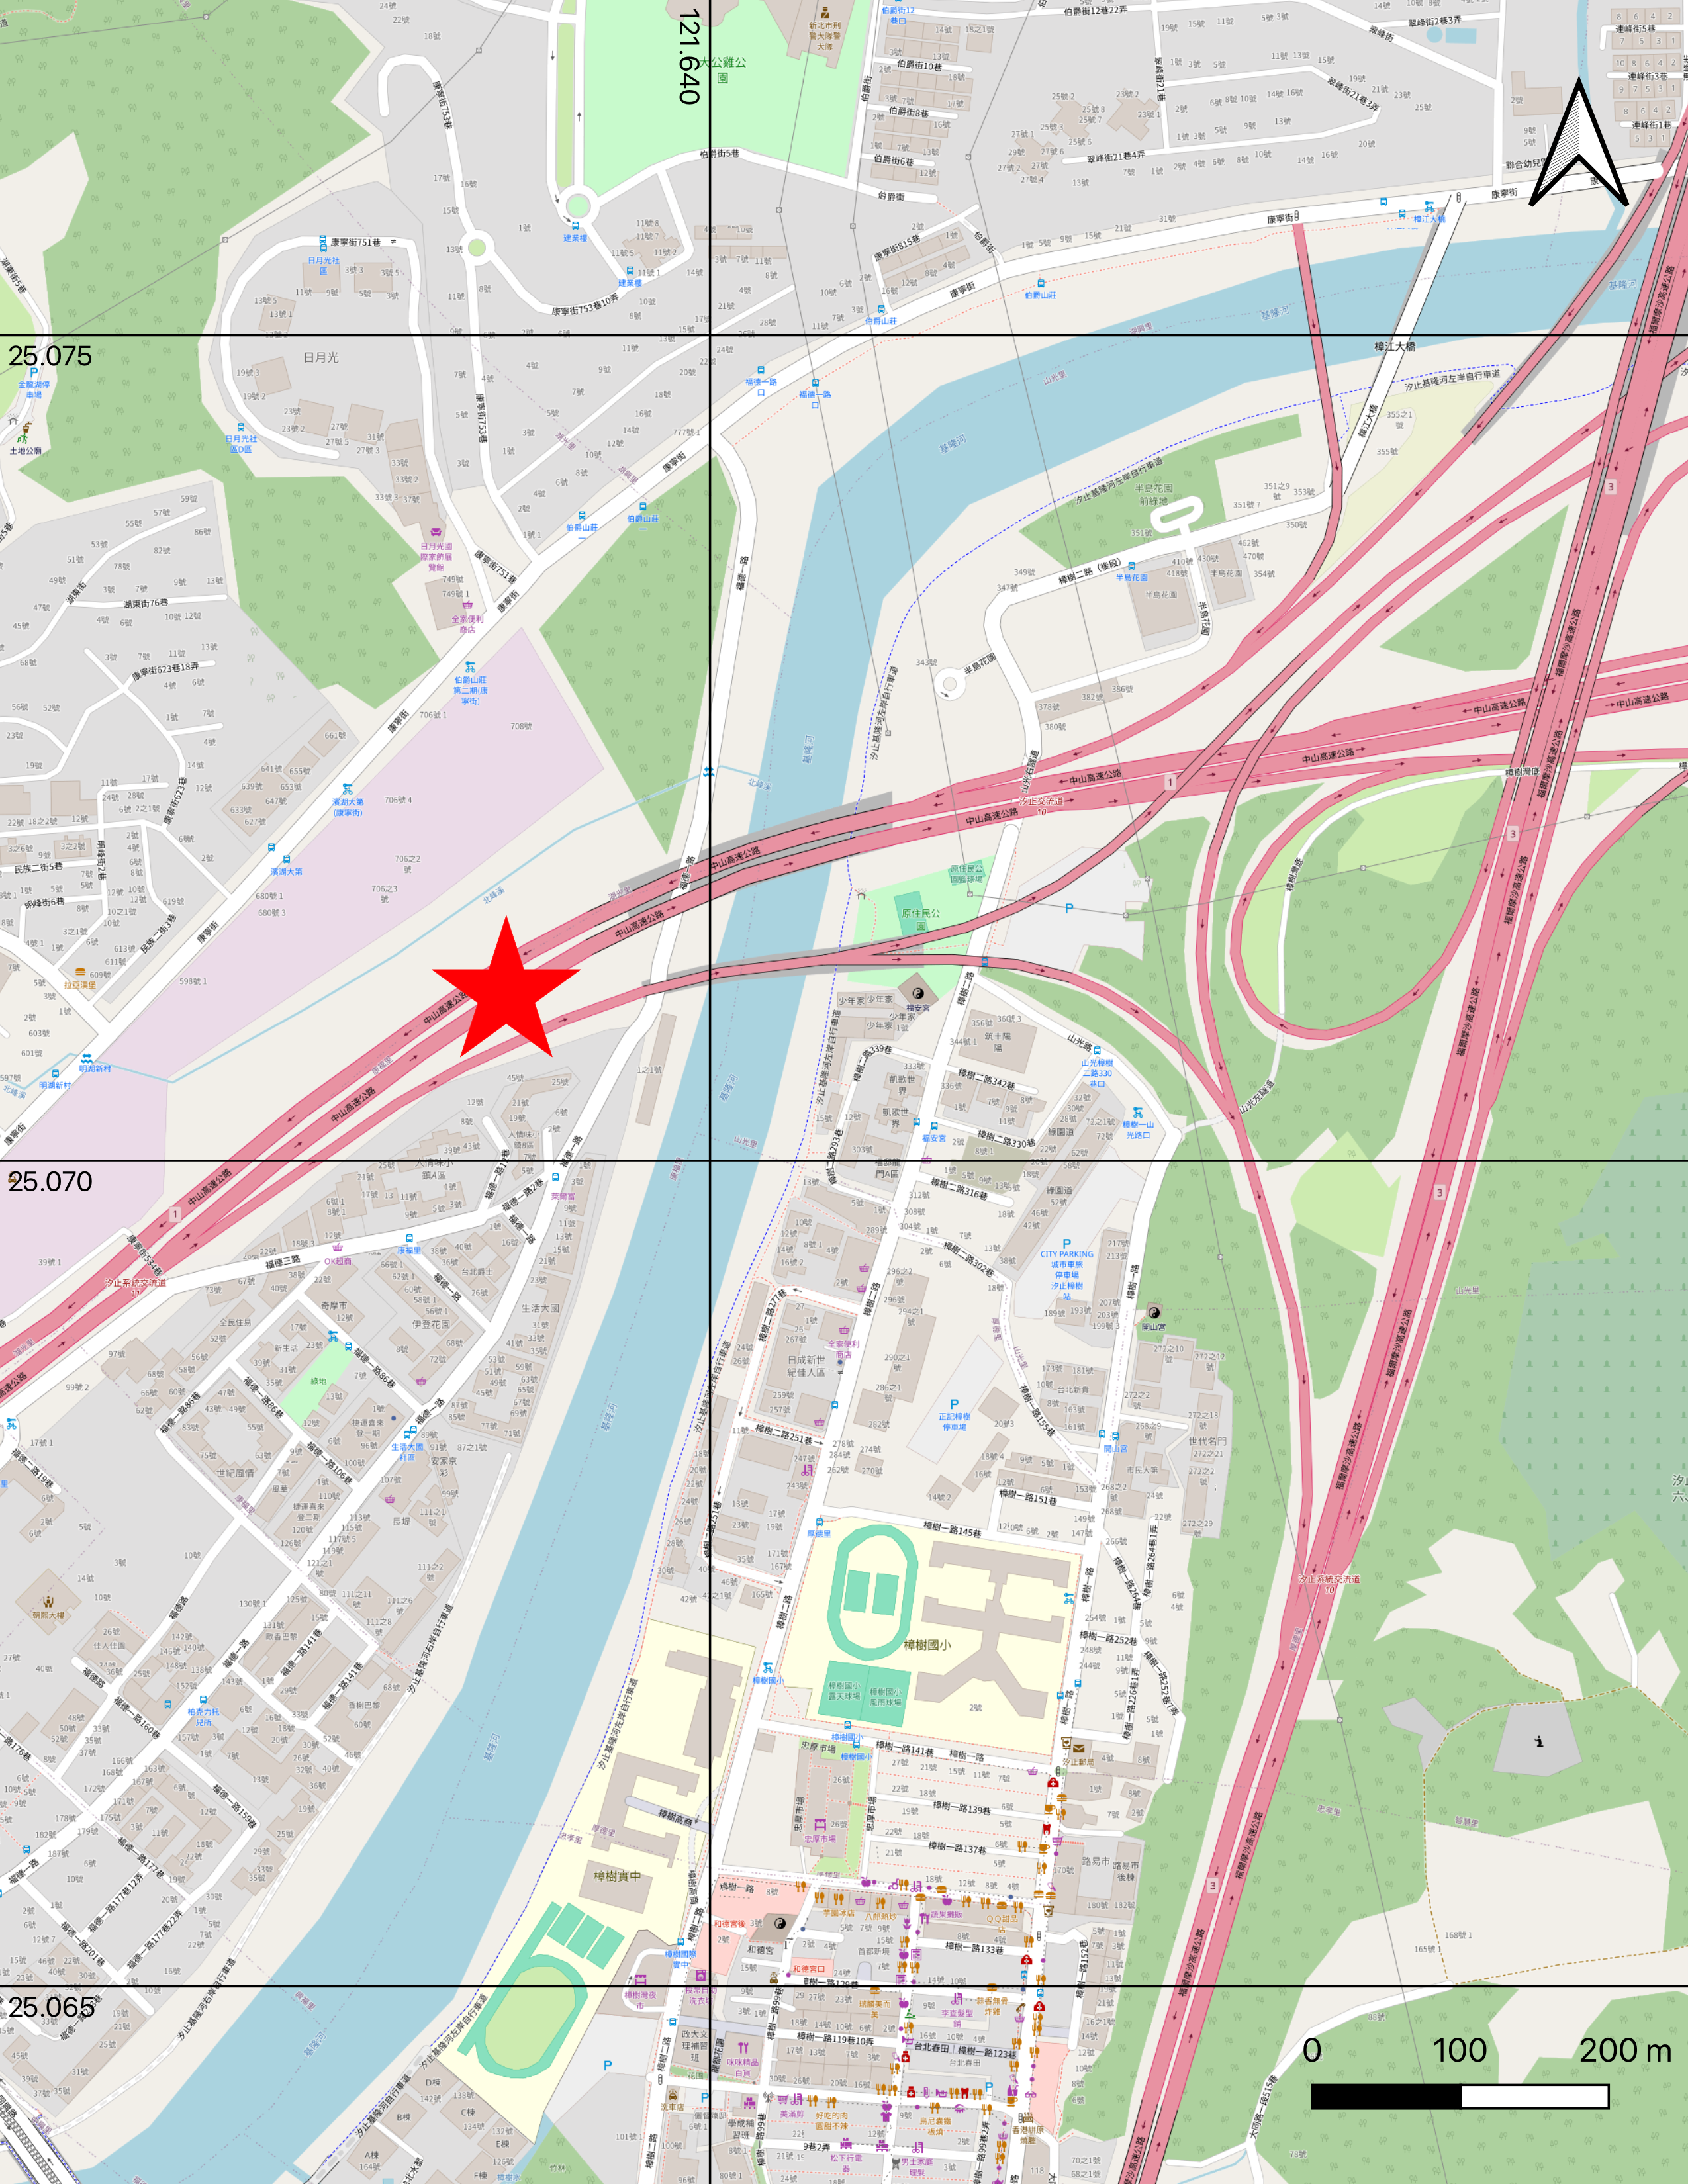
\includegraphics[width=0.95\linewidth]{figures/cases/case1_1.png} & 中山高速公路12.1公里附近（汐止系統交流道） & 北上在12公里到7公里之間.汐止系統前~五堵.內線. & 位於新北市汐止區，鄰近台北101東北約10公里，靠近國道一號汐止交流道，附近有基隆河，屬於住宅區。 \\ \hline
1-2 & 
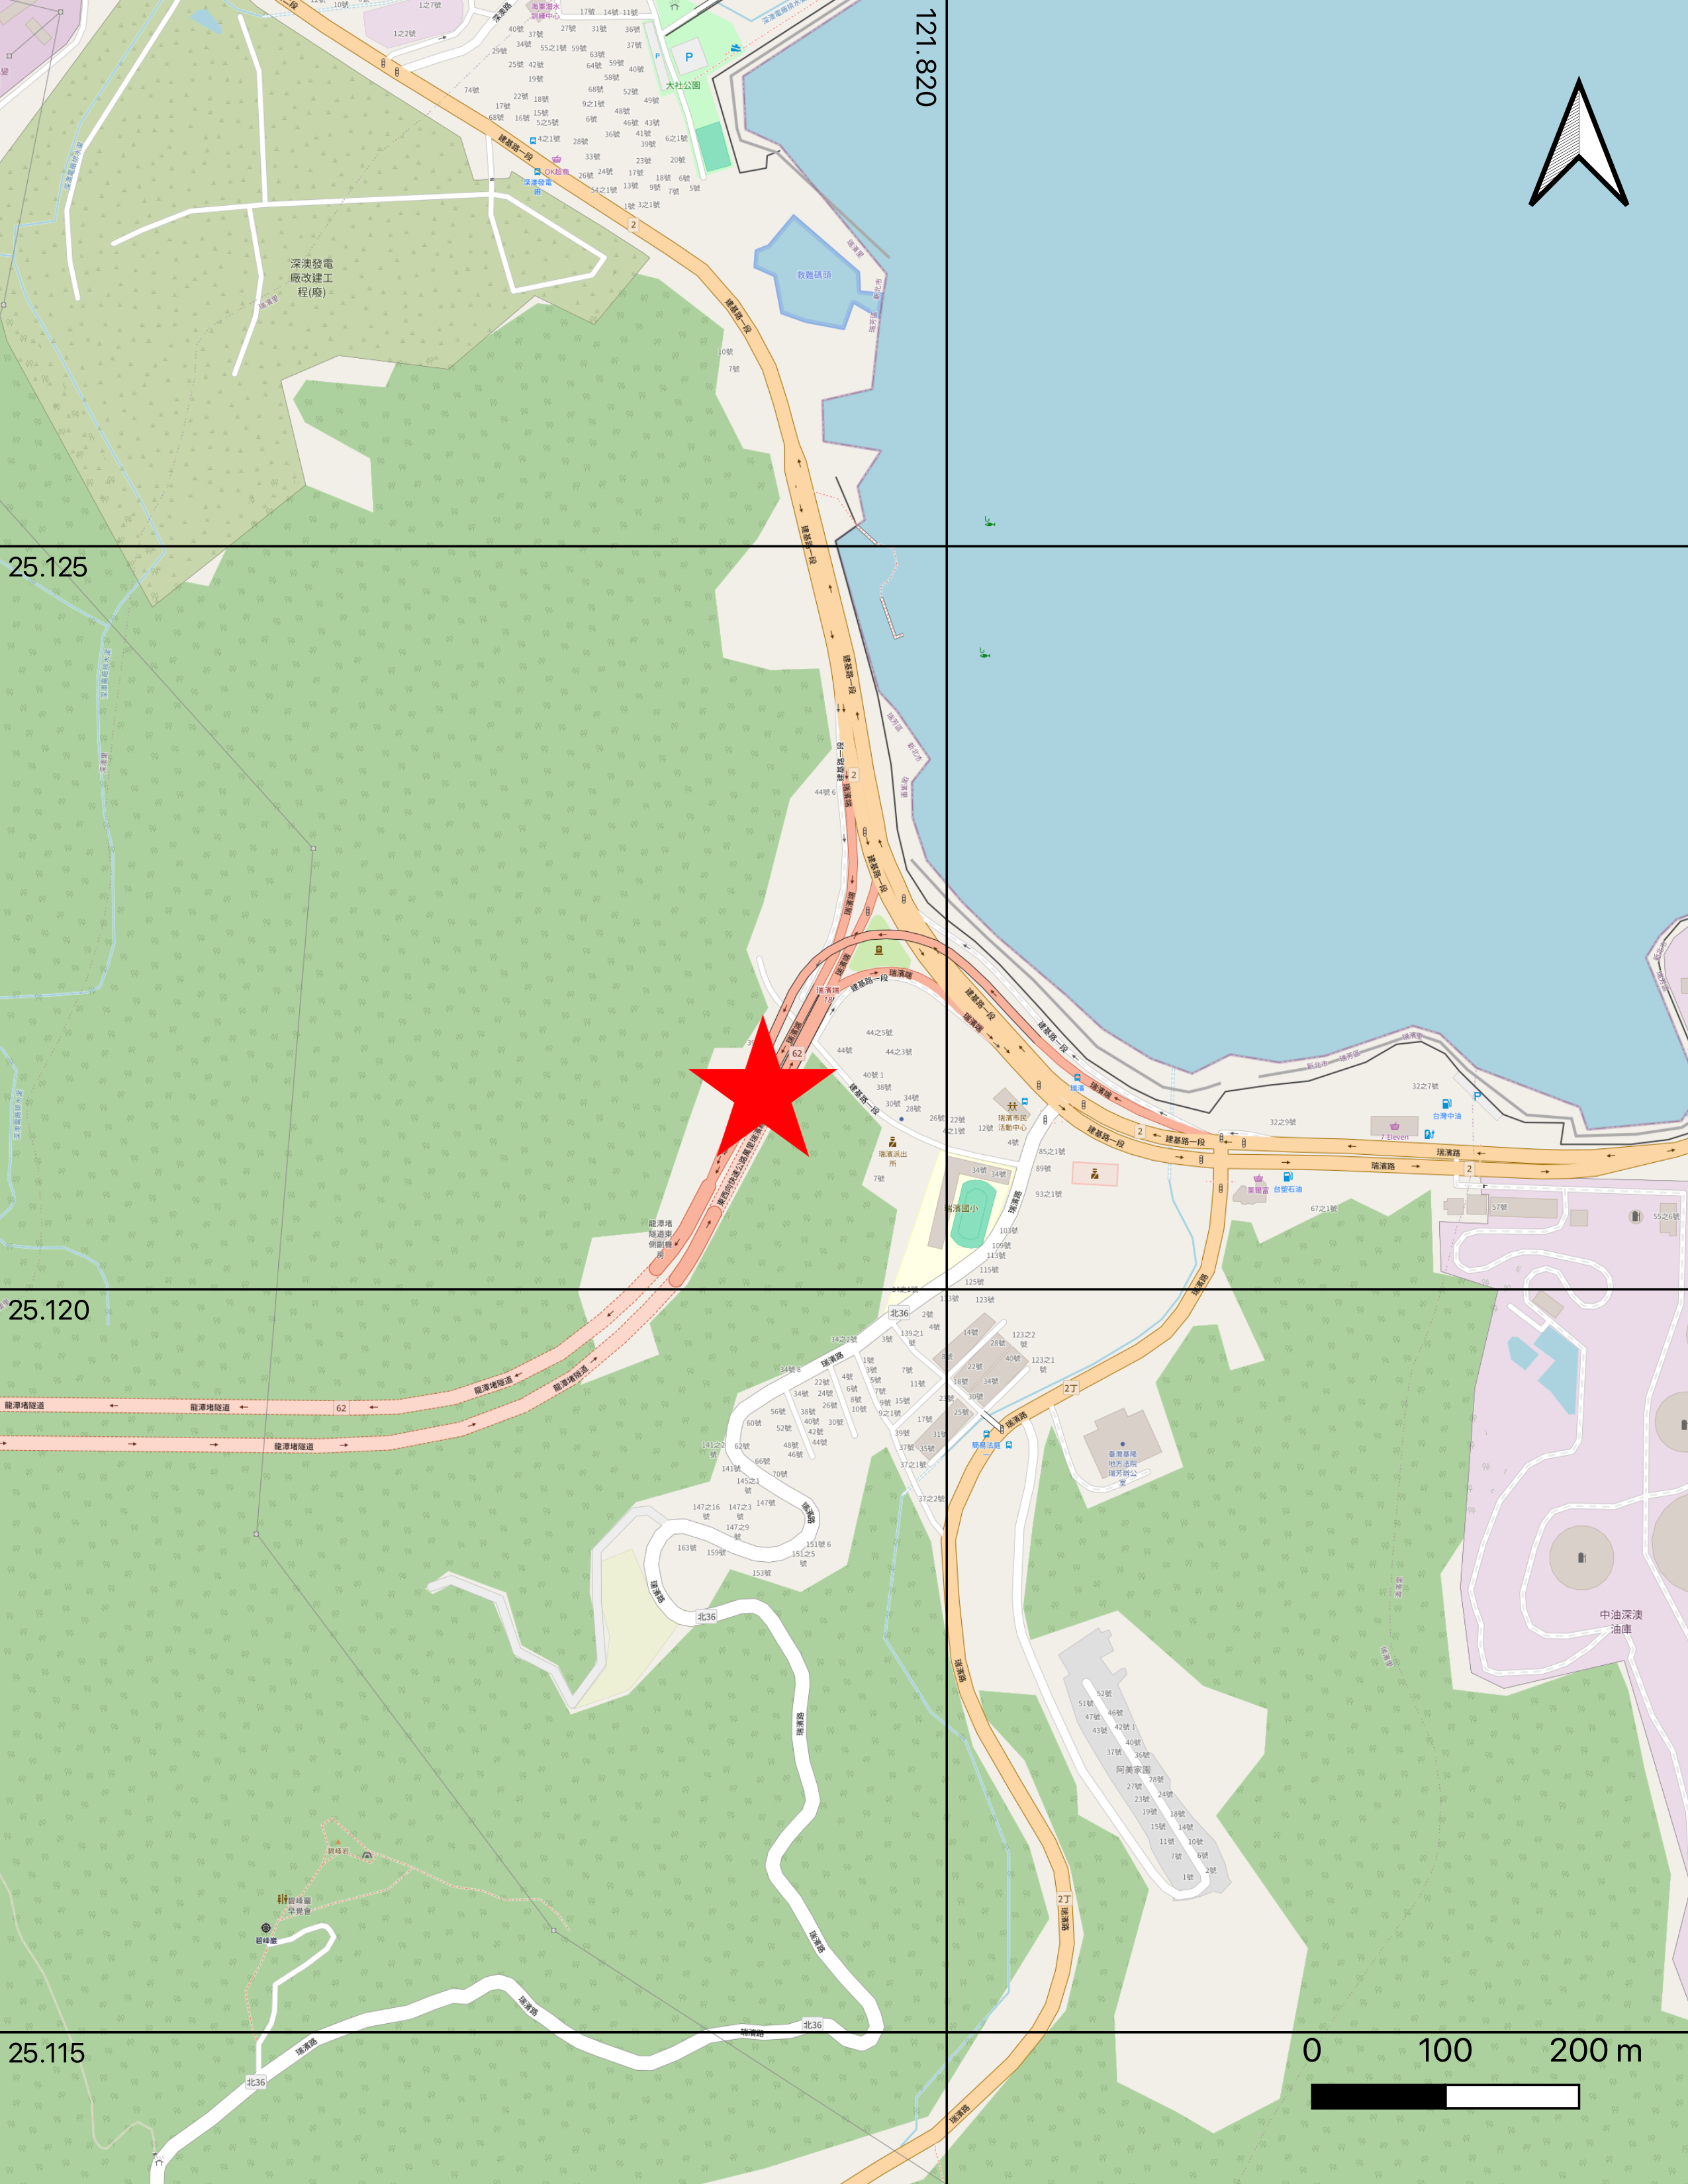
\includegraphics[width=0.95\linewidth]{figures/cases/case1_2.png} & 新北市瑞芳區瑞濱路（龍潭堵隧道） & 西行在18.4公里到17.3公里之間.龍潭堵隧道 & 位於新北市瑞芳區，靠近九份老街東南約300公尺，鄰近基山街和輔仁路交會處，接近基隆河岸，屬於觀光區。 \\ \hline
1-3 &
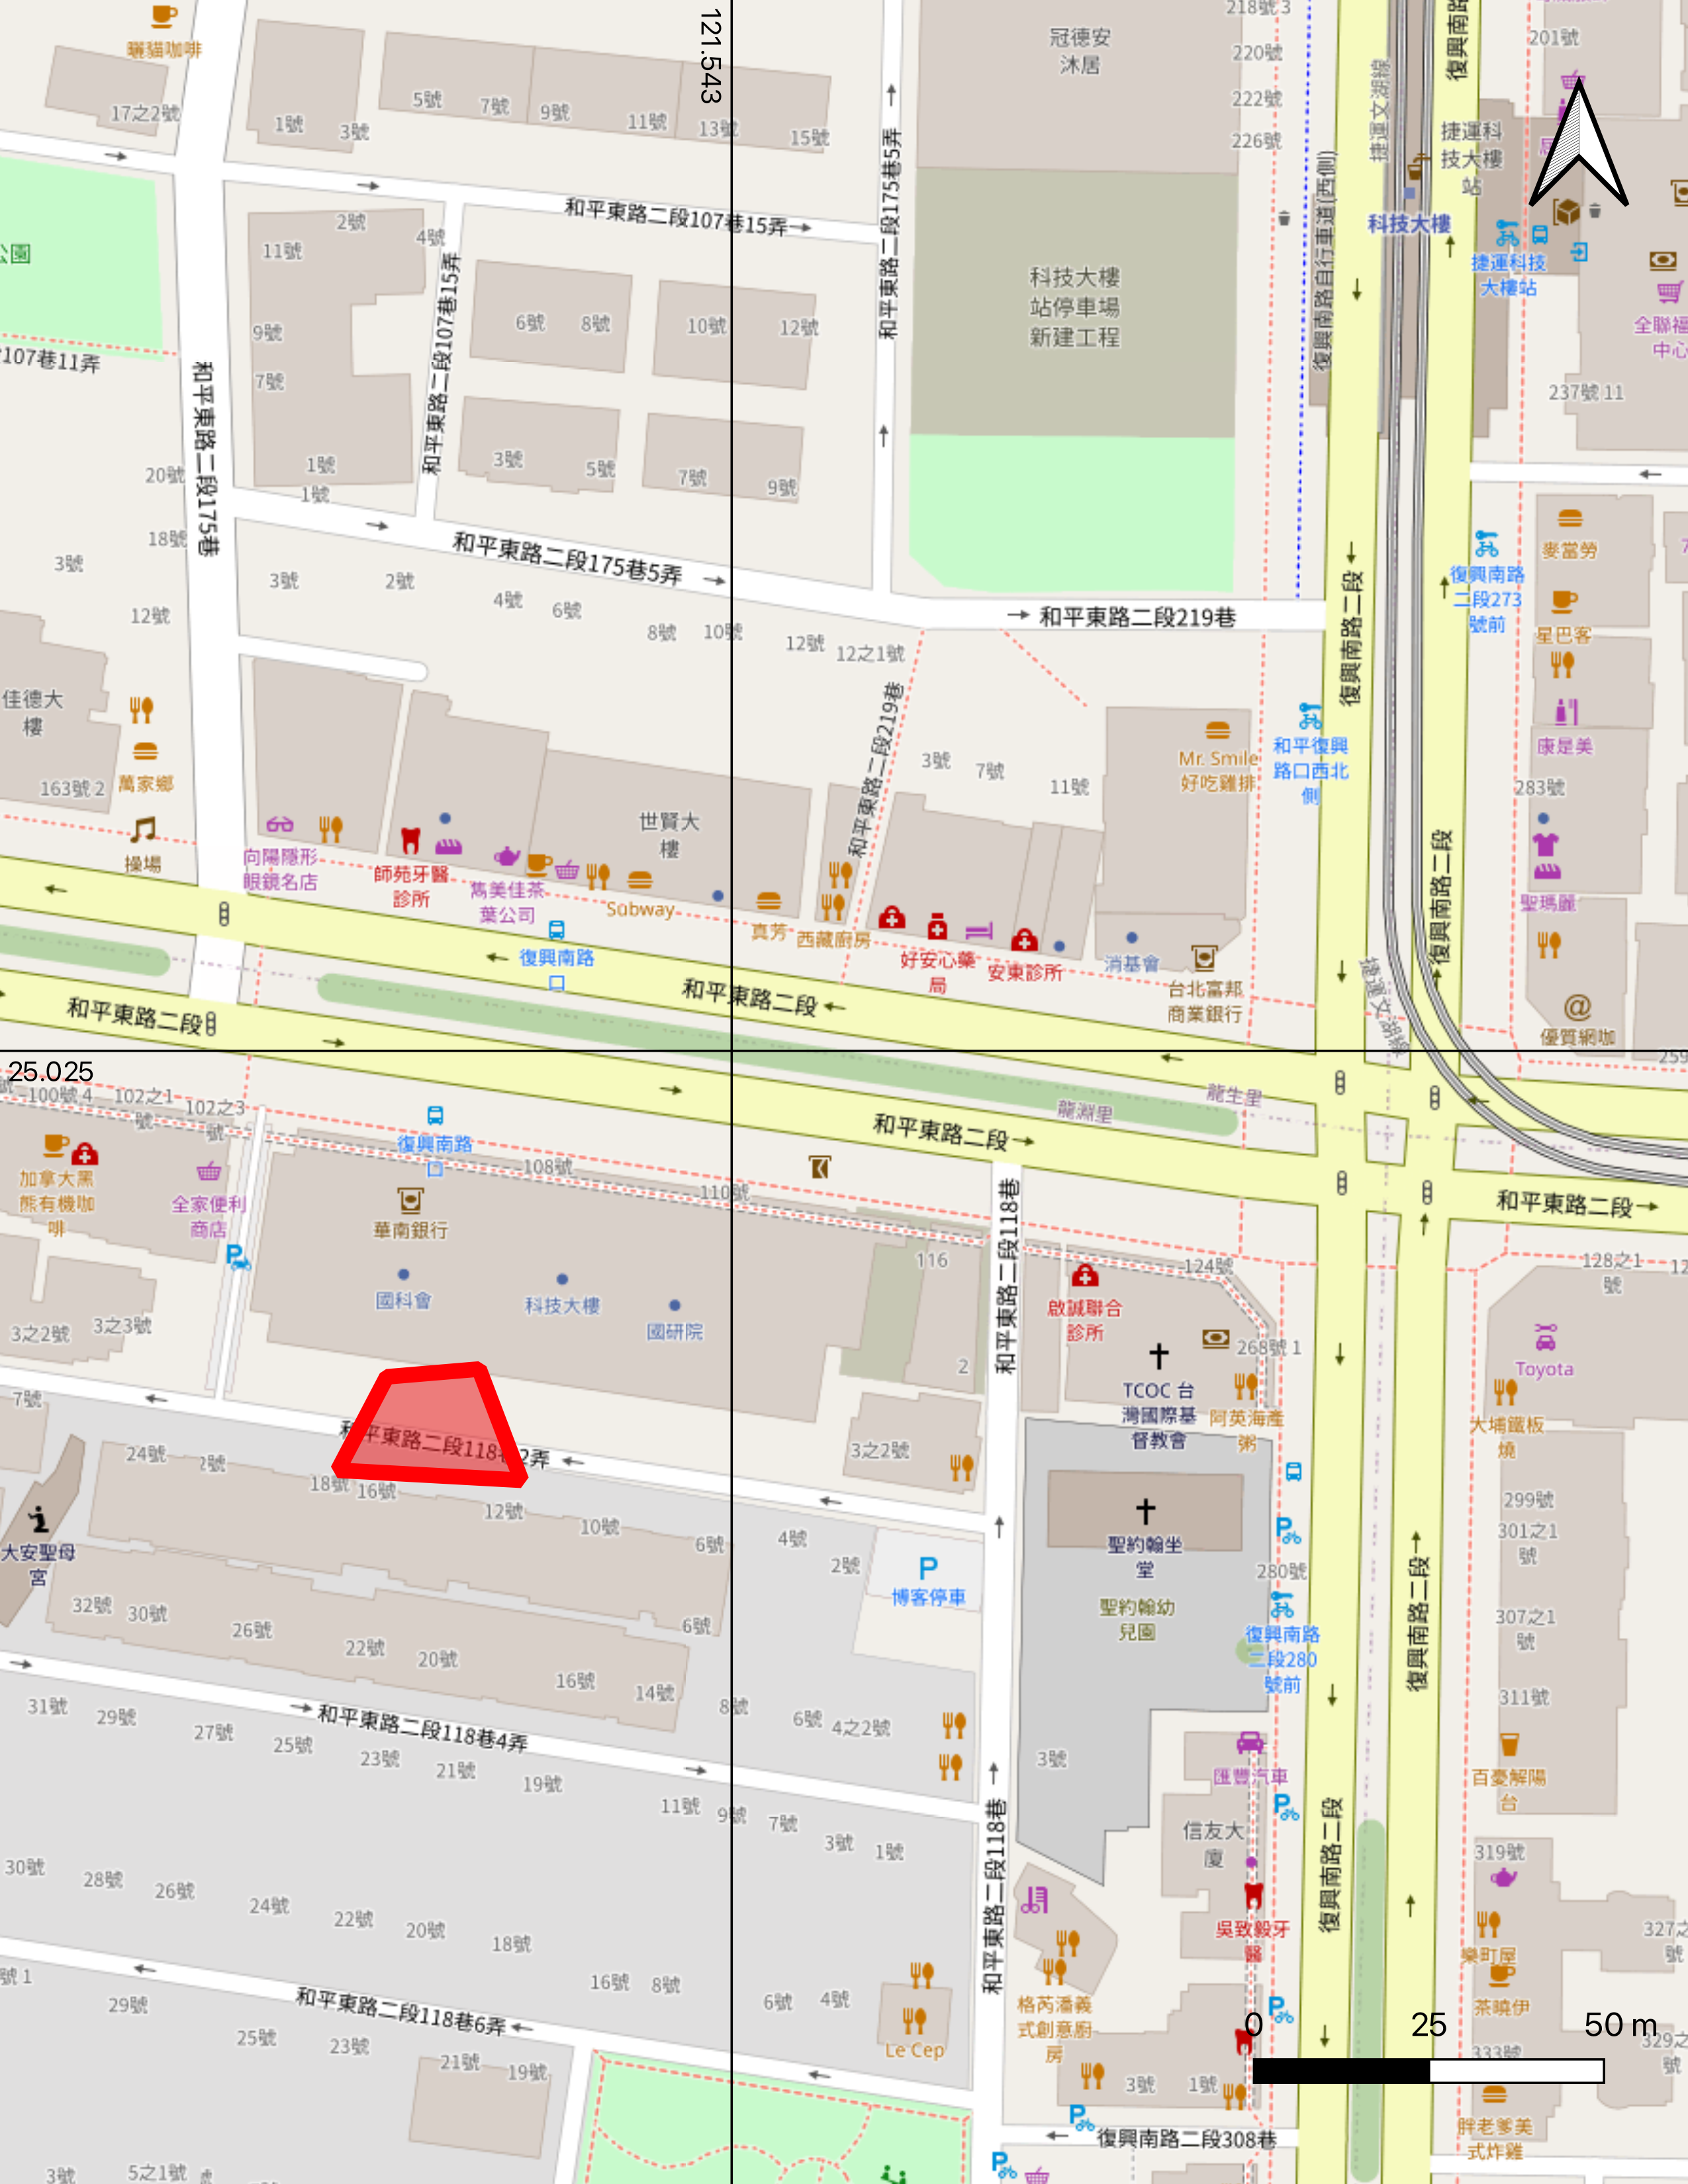
\includegraphics[width=0.95\linewidth]{figures/cases/case1_3.png} & 在臺北市大安區和平東路二段118巷2弄（科技部附近） & 和平東路二段118巷2弄16號 & 位於台北市大安區，鄰近台北101東北約1公里，靠近信義路四段與基隆路交叉口，臨近大安森林公園，屬於商業區。 \\ \hline
1-4 &
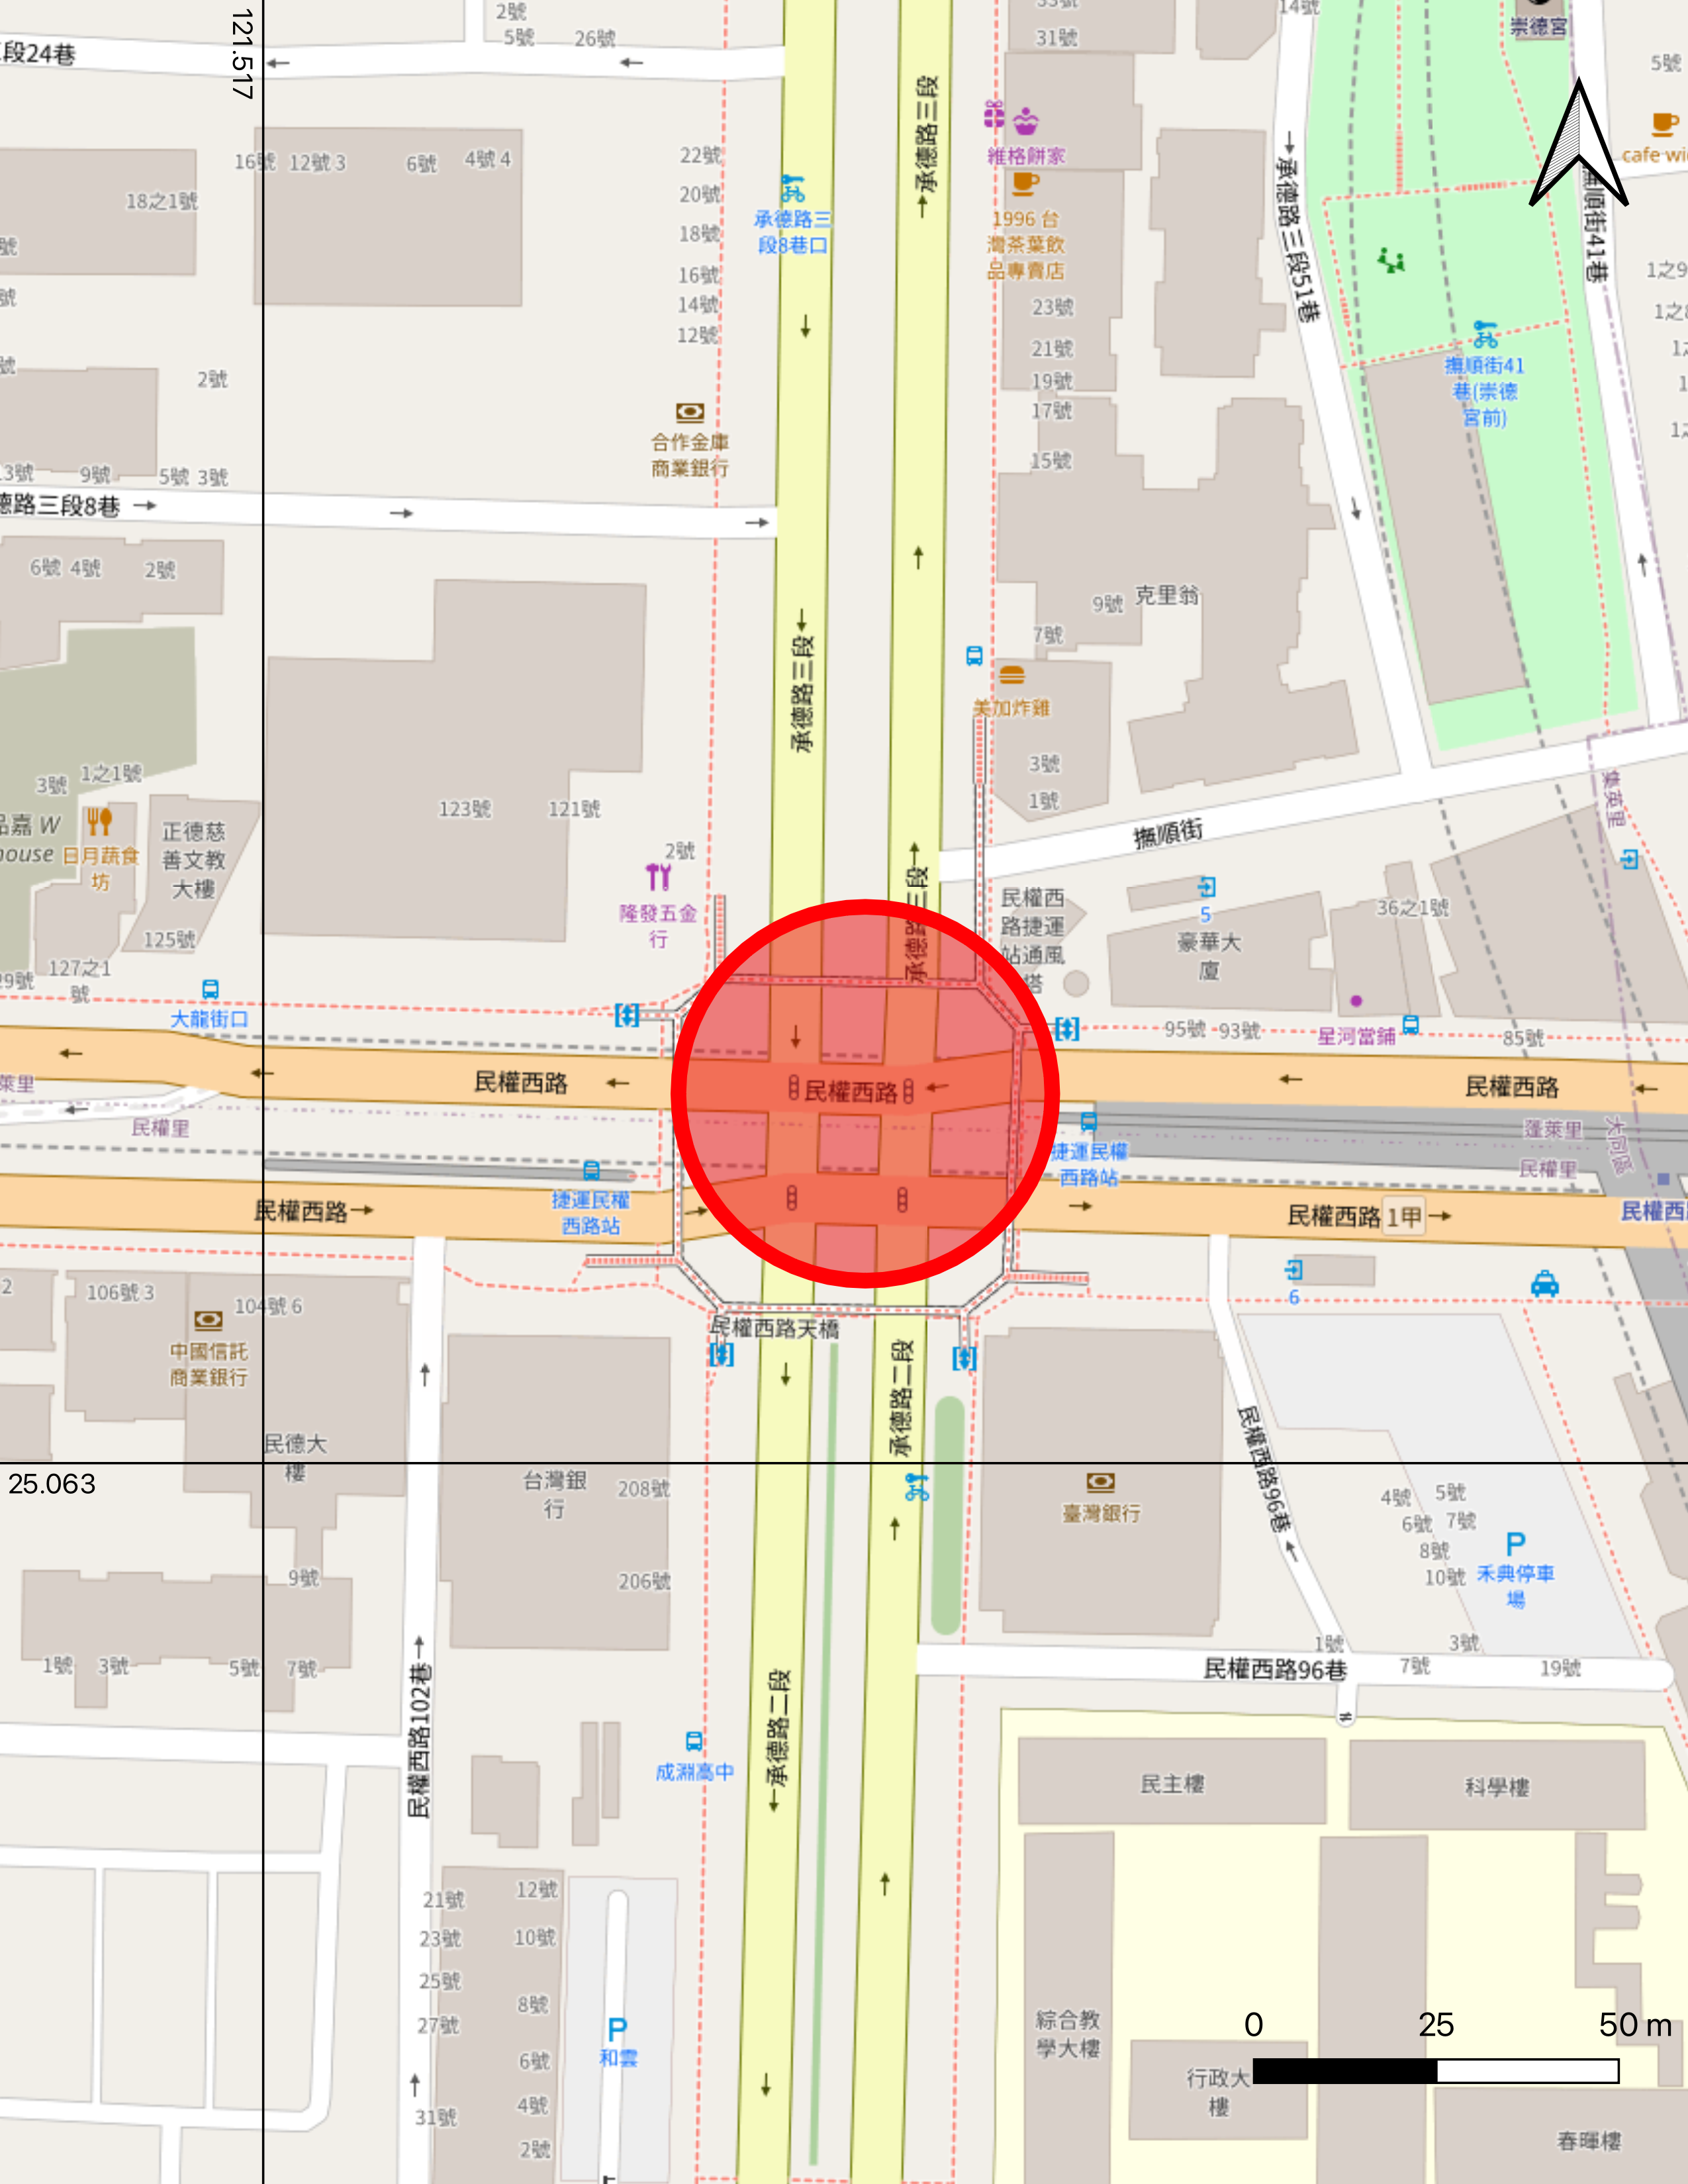
\includegraphics[width=0.95\linewidth]{figures/cases/case1_4.png} & 在臺北市大同區民權西路路口（捷運民權西路站附近）  & 承德路二段+民權西路口 & 位於台北市中正區，靠近台北車站東南約300公尺，鄰近忠孝西路與館前路交會處，周圍為商業區中心。 \\ \hline
1-5 &
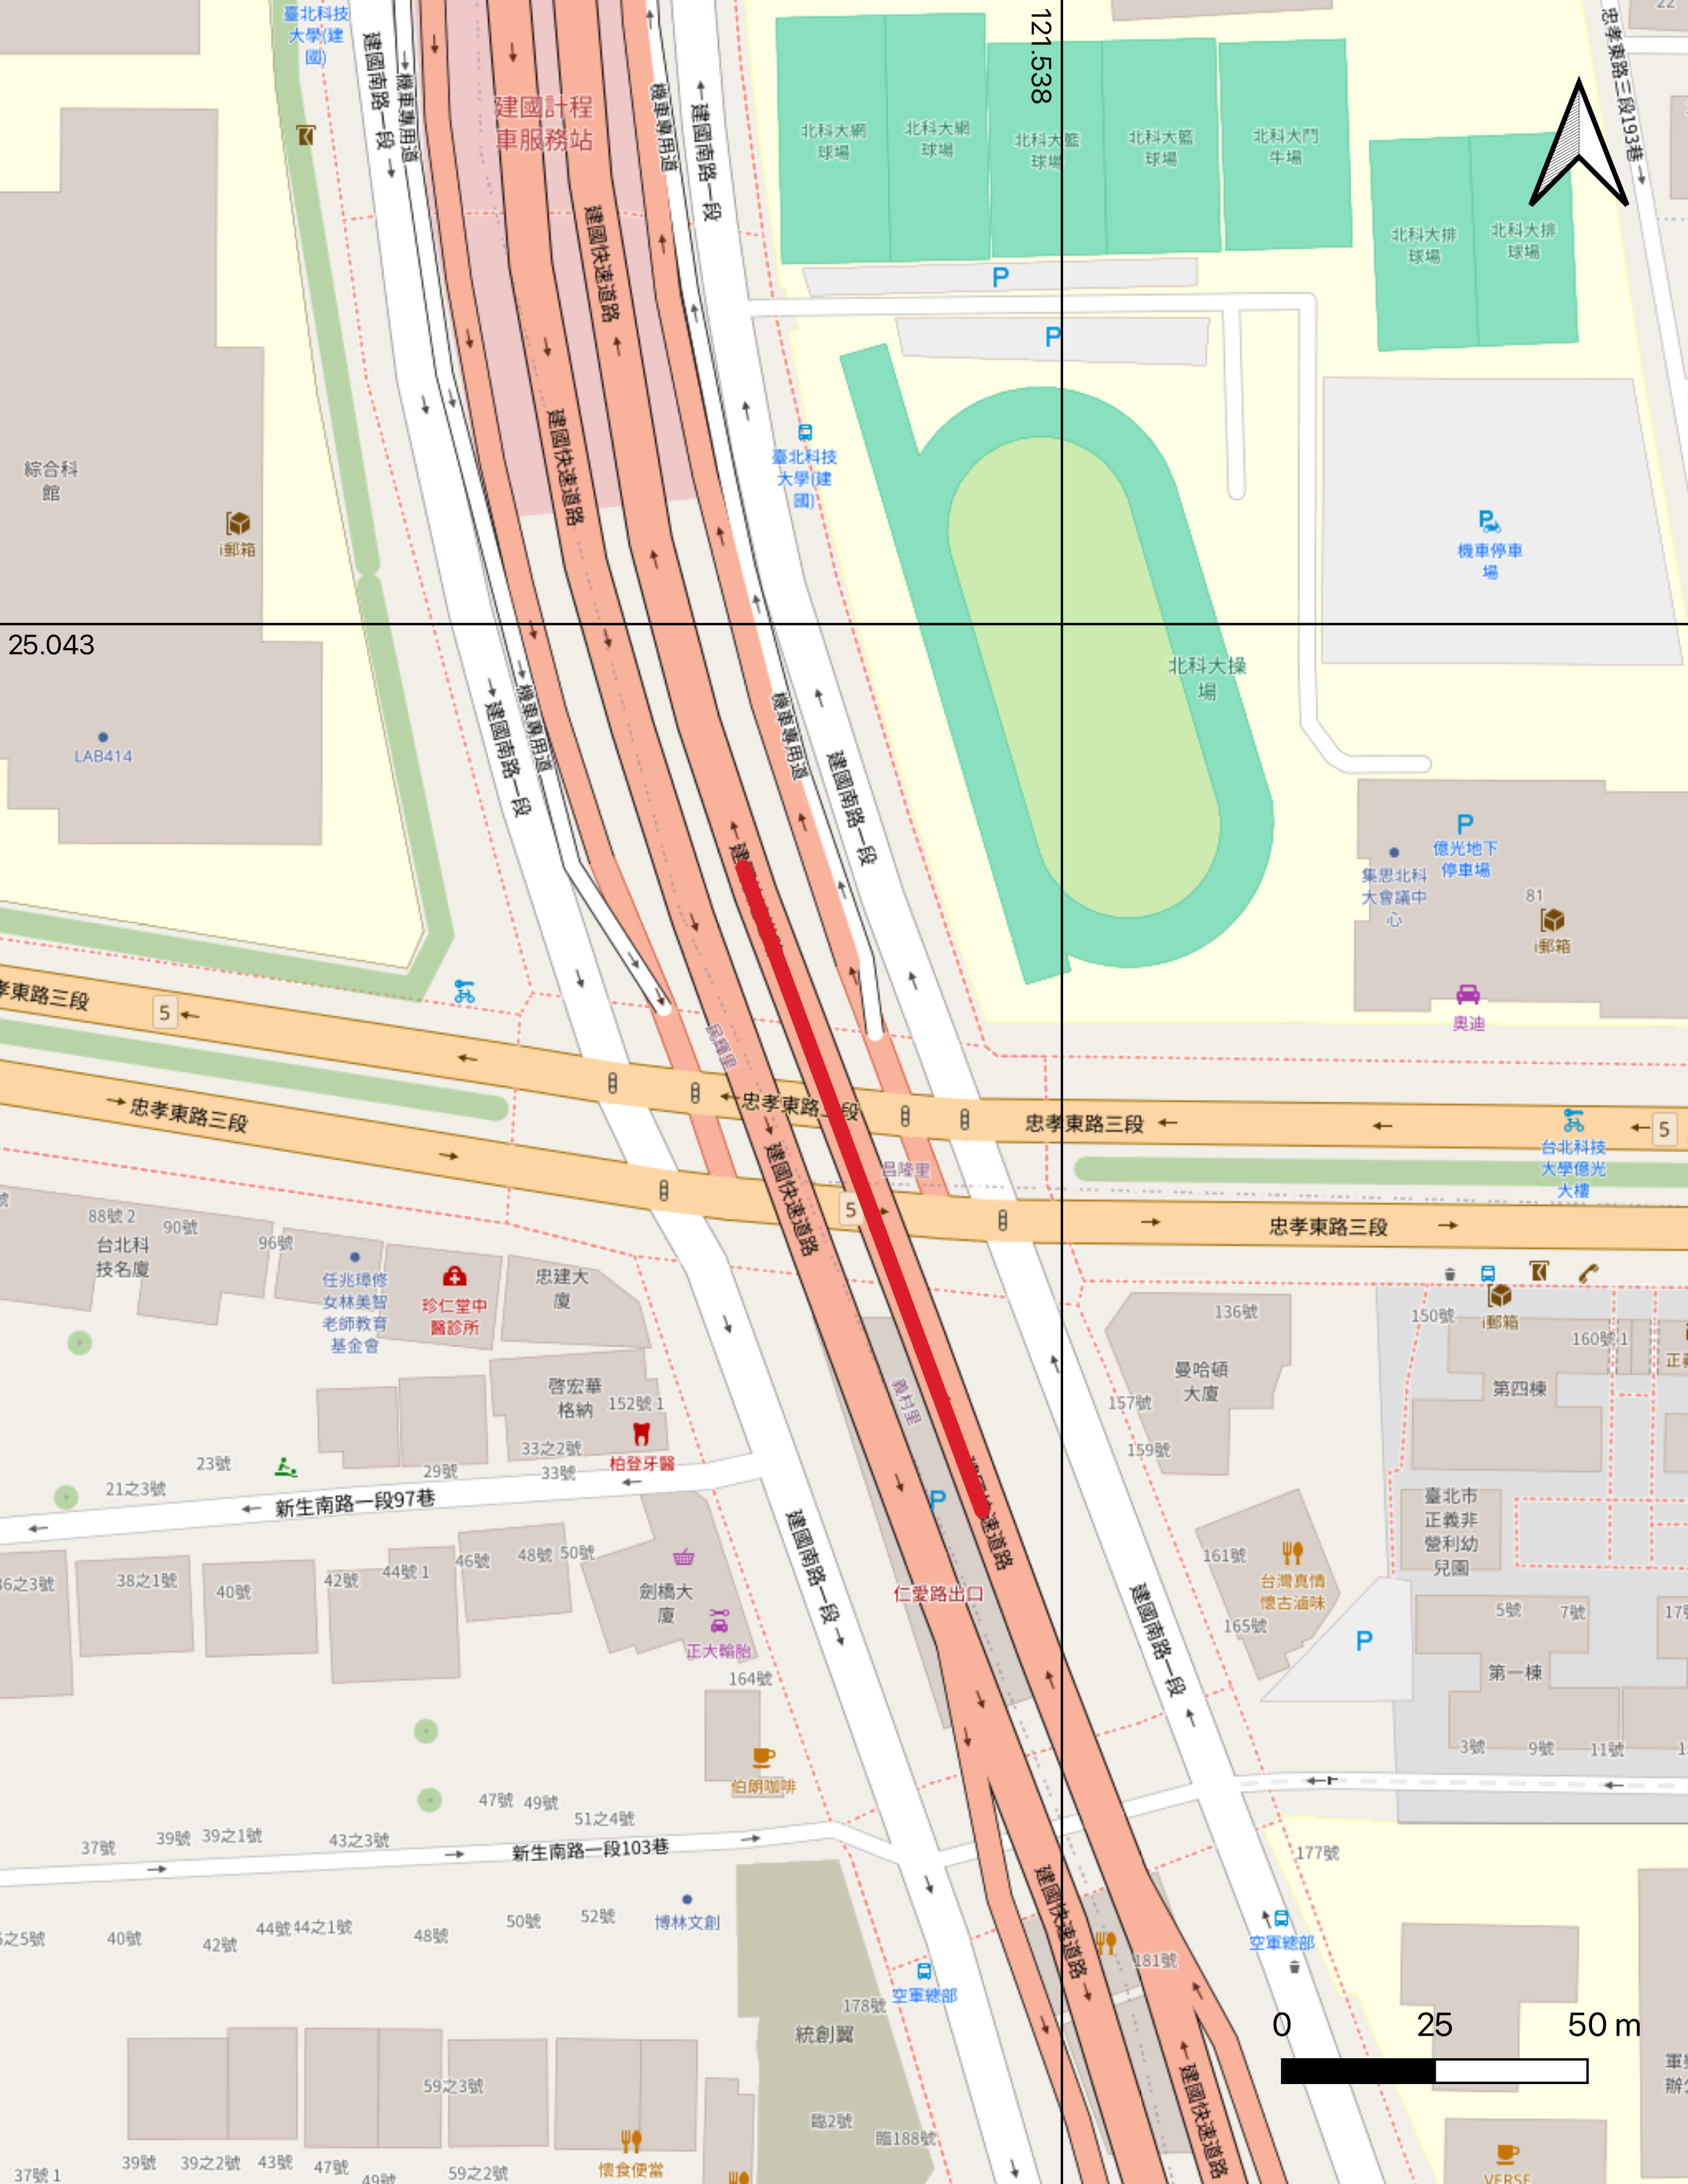
\includegraphics[width=0.95\linewidth]{figures/cases/case1_5.png} & 在臺北市大安區建國南北快速道路上（忠孝東路三段上方） & 建高往北.忠孝東路上方 & 位於台北市大安區，鄰近台北101東北約1公里，靠近信義路和復興南路交會處，接近大安森林公園，屬於商業區。 \\ \hline
1-6 & 
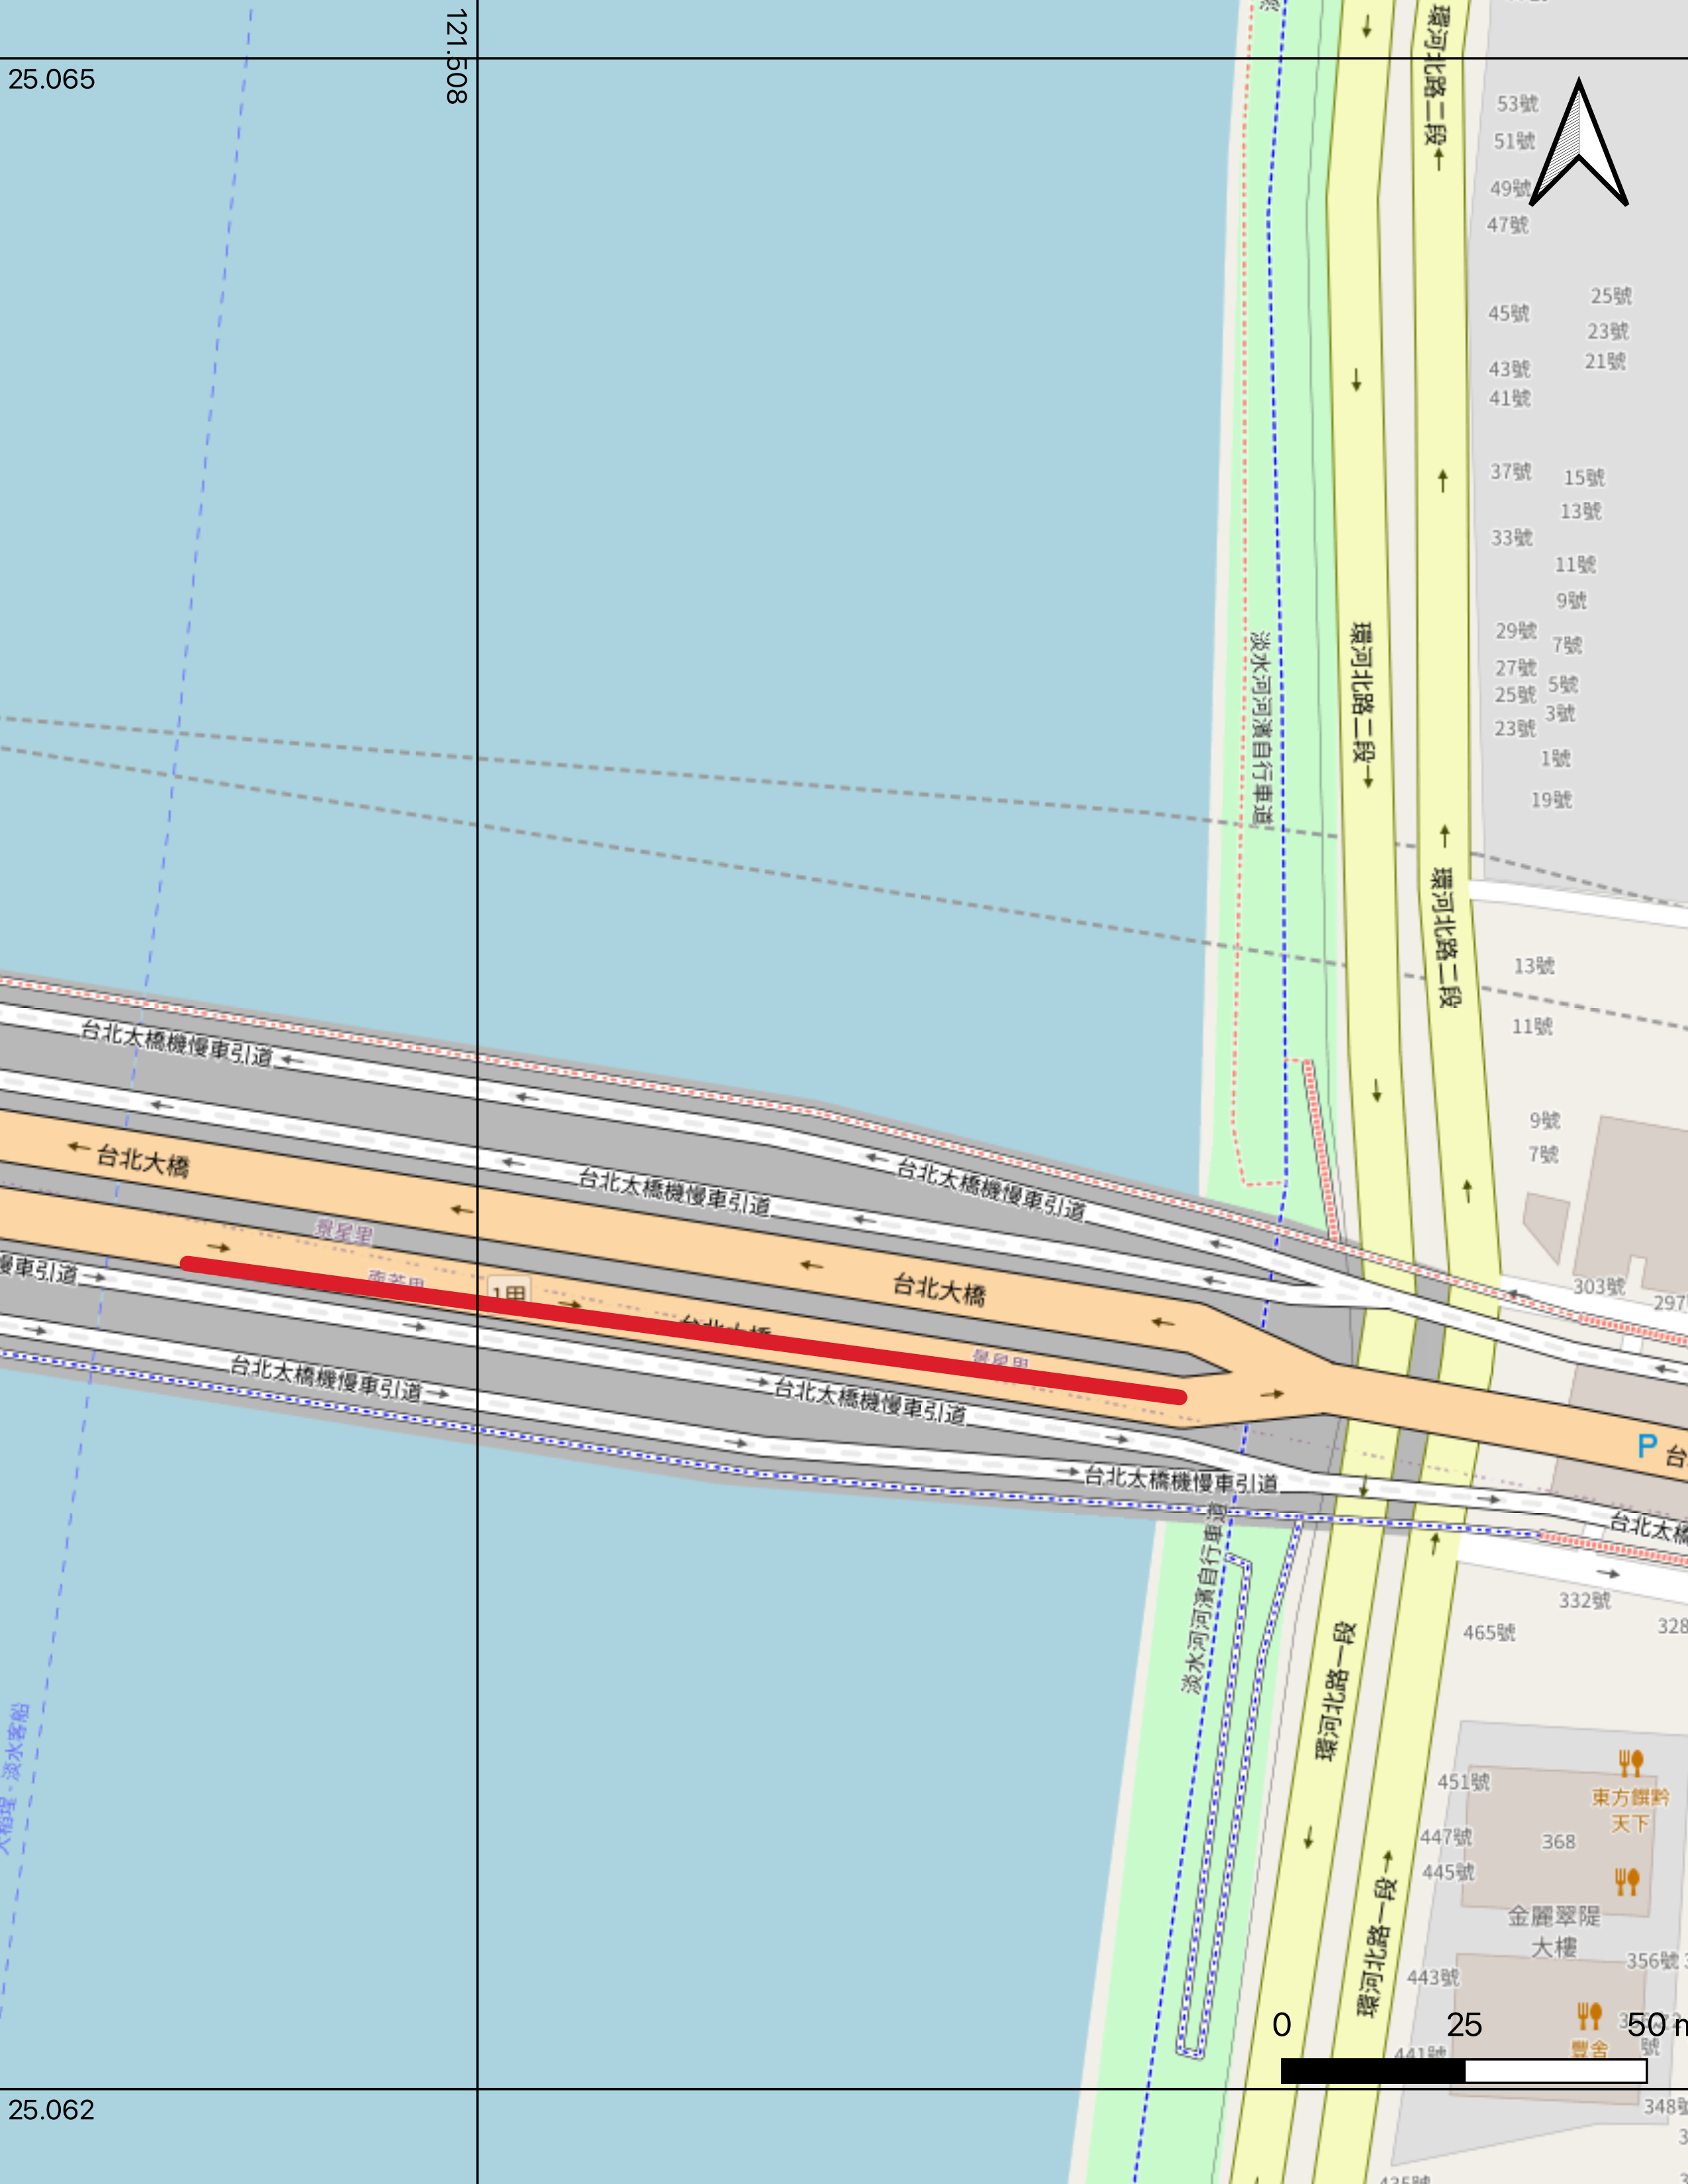
\includegraphics[width=0.95\linewidth]{figures/cases/case1_6.png} & 在台北大橋 & 台北橋往台北 & 位於台北市信義區，鄰近台北101東北約300公尺，靠近信義路五段與松智路交會處，臨近基隆河岸，屬於商業區中心。 \\ \hline
2-1 &
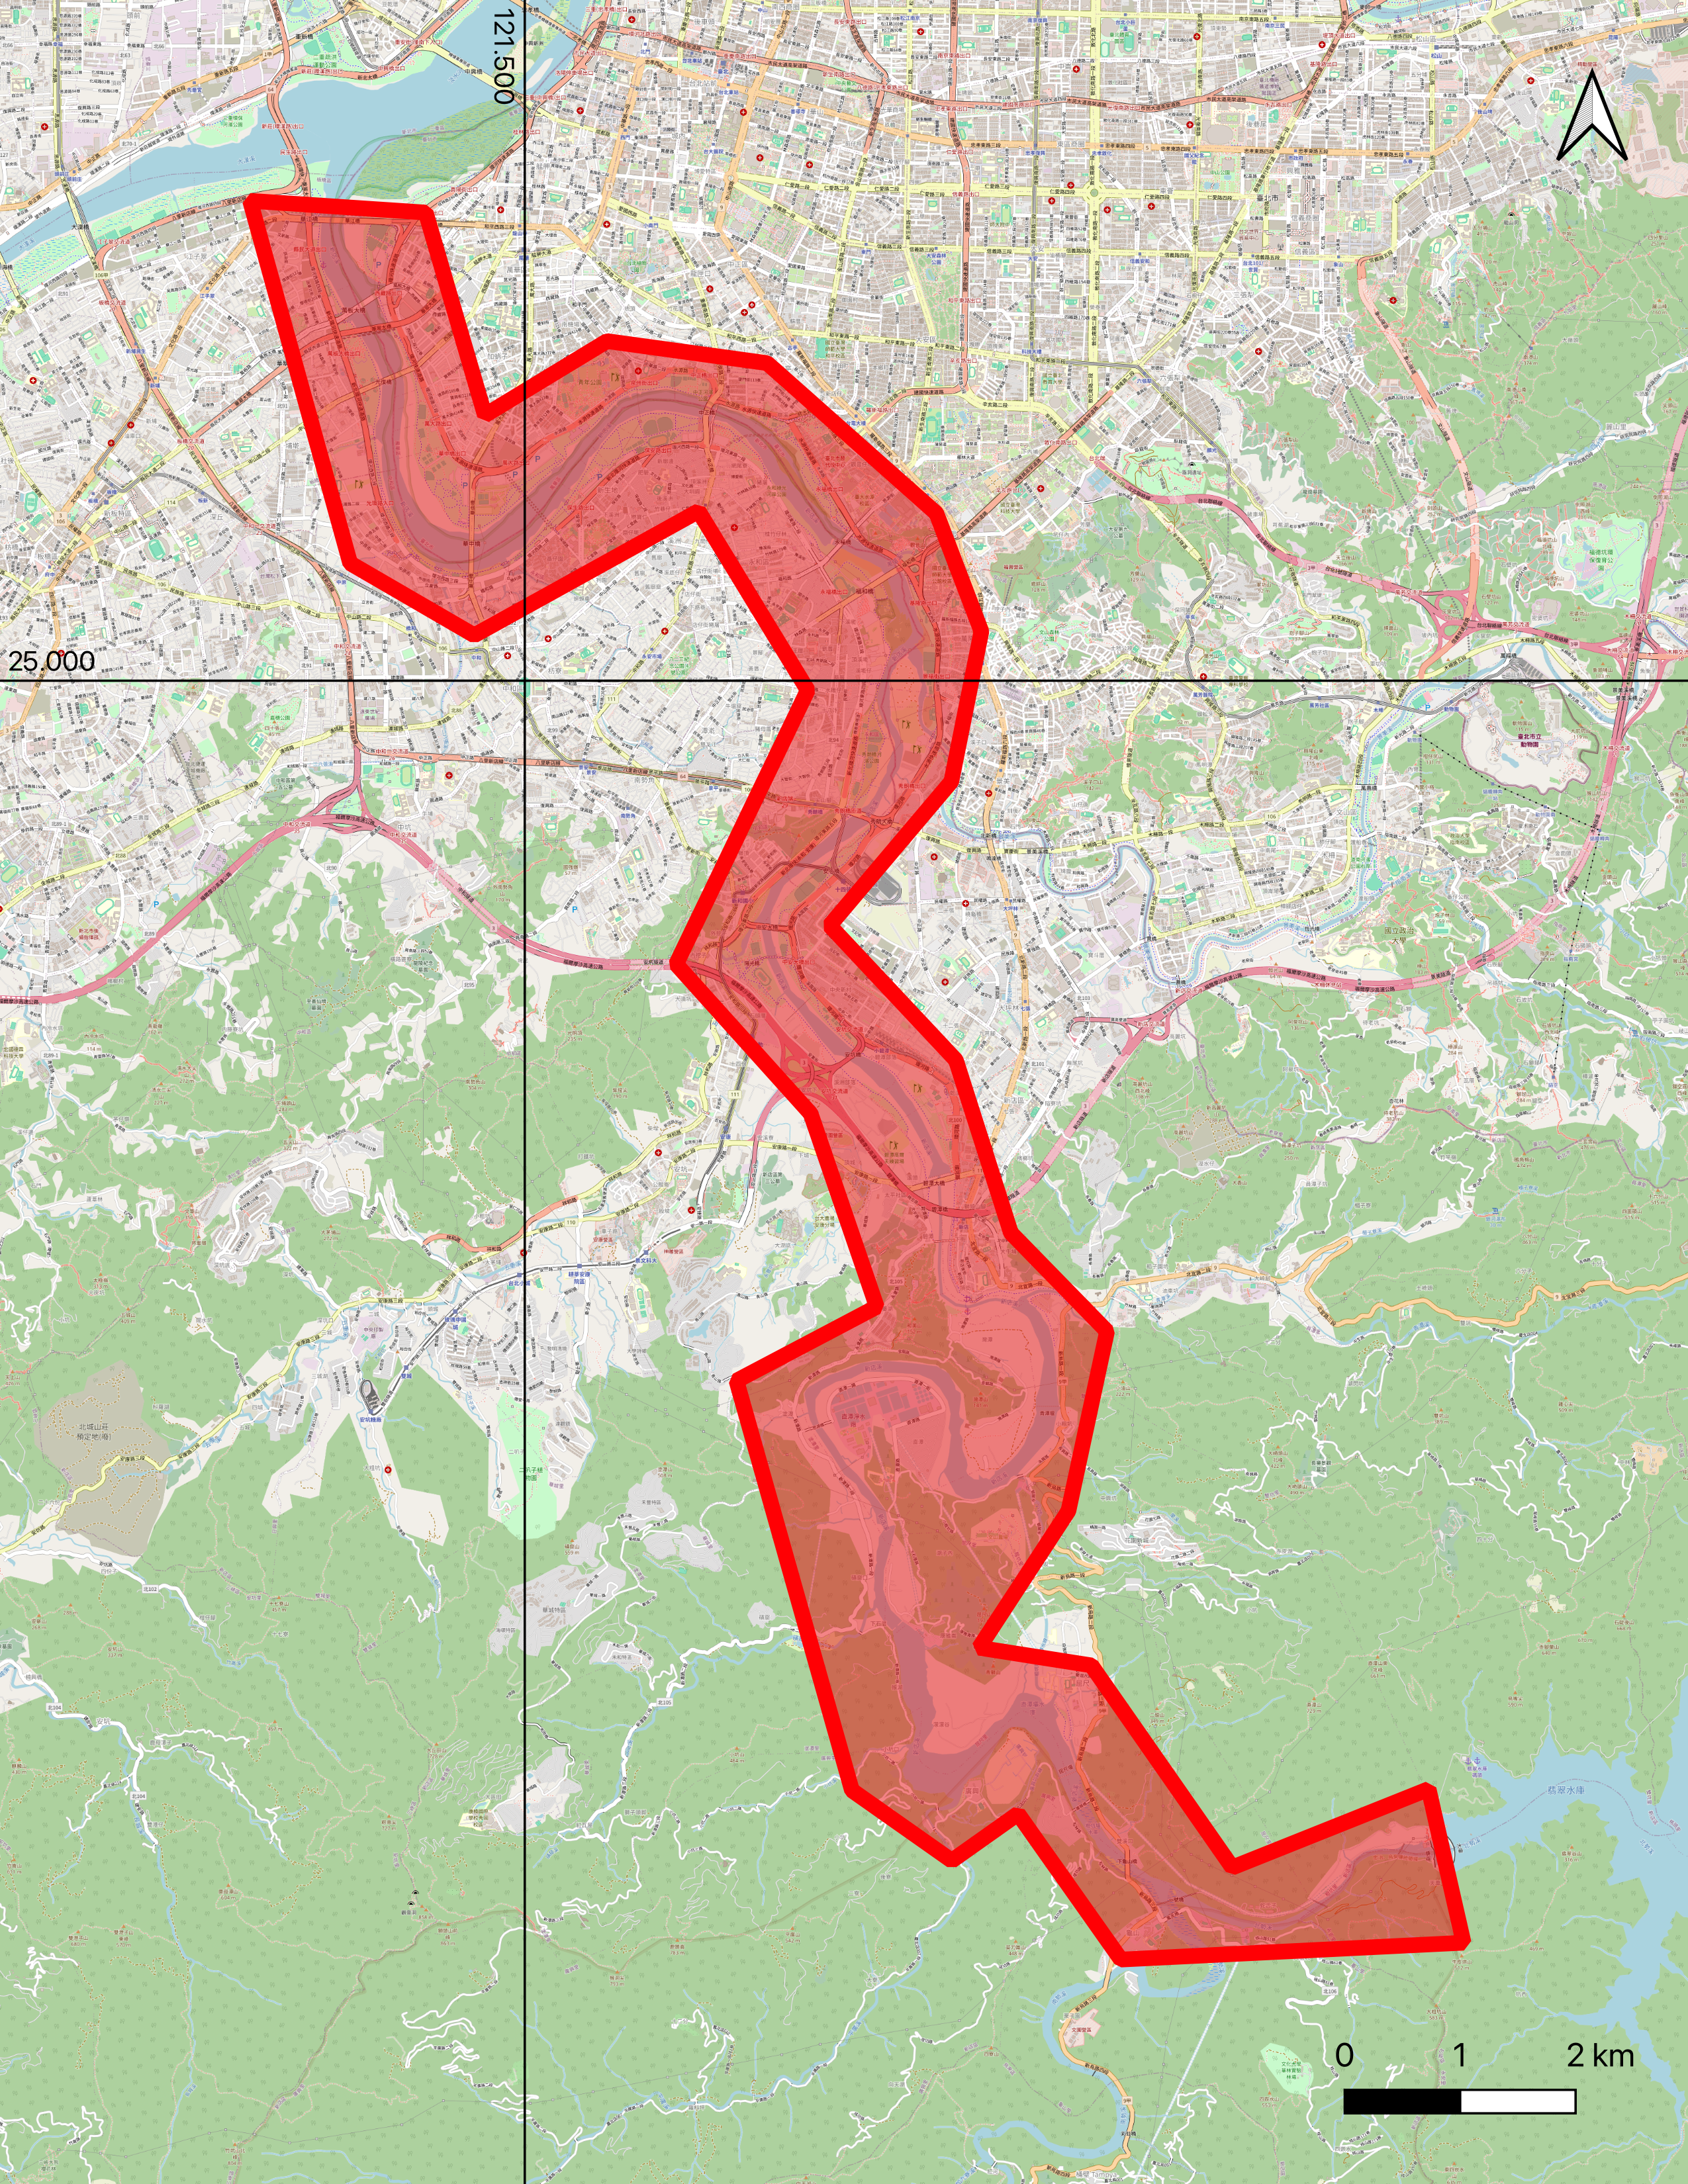
\includegraphics[width=0.95\linewidth]{figures/cases/case2_1.png} & 在新北市石碇區、中和區、板橋區、永和區、臺北市文山區、臺北市萬華區、臺北市中正區和新店區淡水河河畔 & 水庫下游北勢溪、新店溪 & 位於新北市中和區，鄰近中和環球購物中心東北約1公里，靠近中山路與中正路交會處，臨近新店溪沿岸，屬於都市住宅區。 \\ \hline
2-2 &
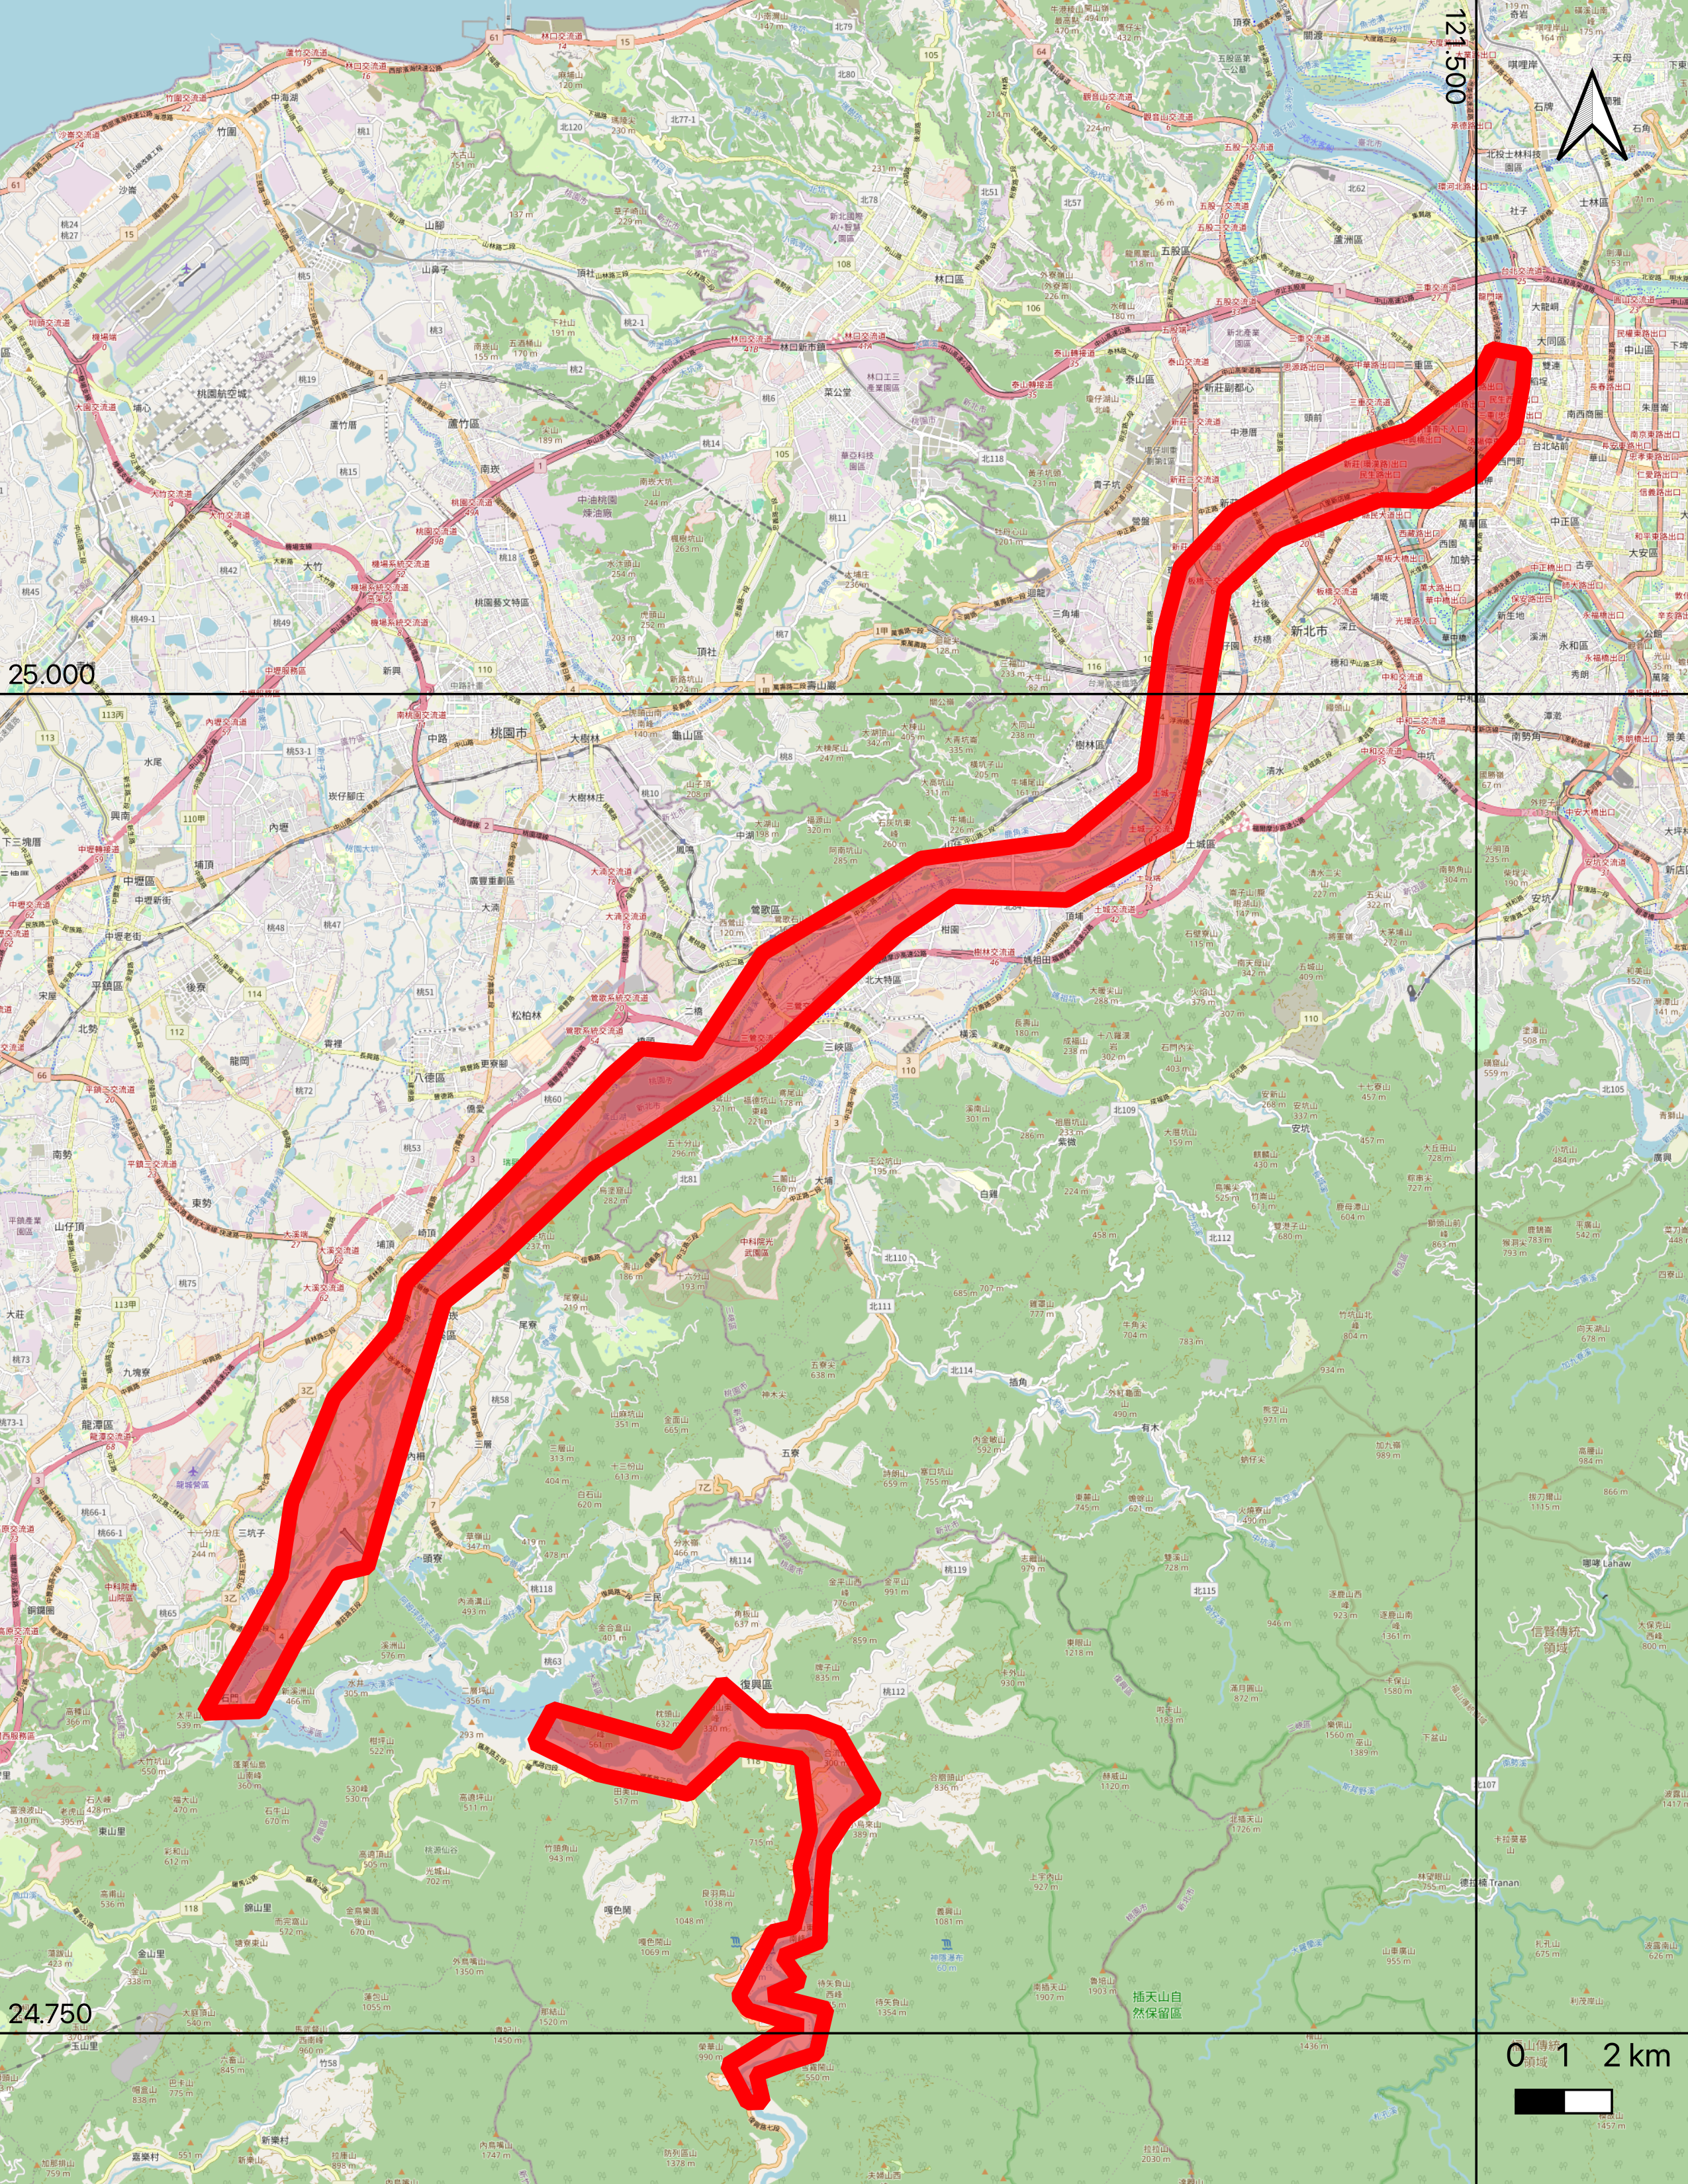
\includegraphics[width=0.95\linewidth]{figures/cases/case2_2.png} & 在新北市板橋區、臺北市萬華區、新莊區、三重區、桃園市龍潭區、桃園市大溪區、鶯歌區、樹林區、土城區、臺北市大同區和三峽區淡水河河畔 & 水庫下游大漢溪、淡水河 & 位於新竹縣尖石鄉，鄰近新竹市東南約20公里，靠近新竹縣尖石鄉主要道路，周圍為山區地形，位於新竹縣尖石鄉。 \\ \hline
2-3 &
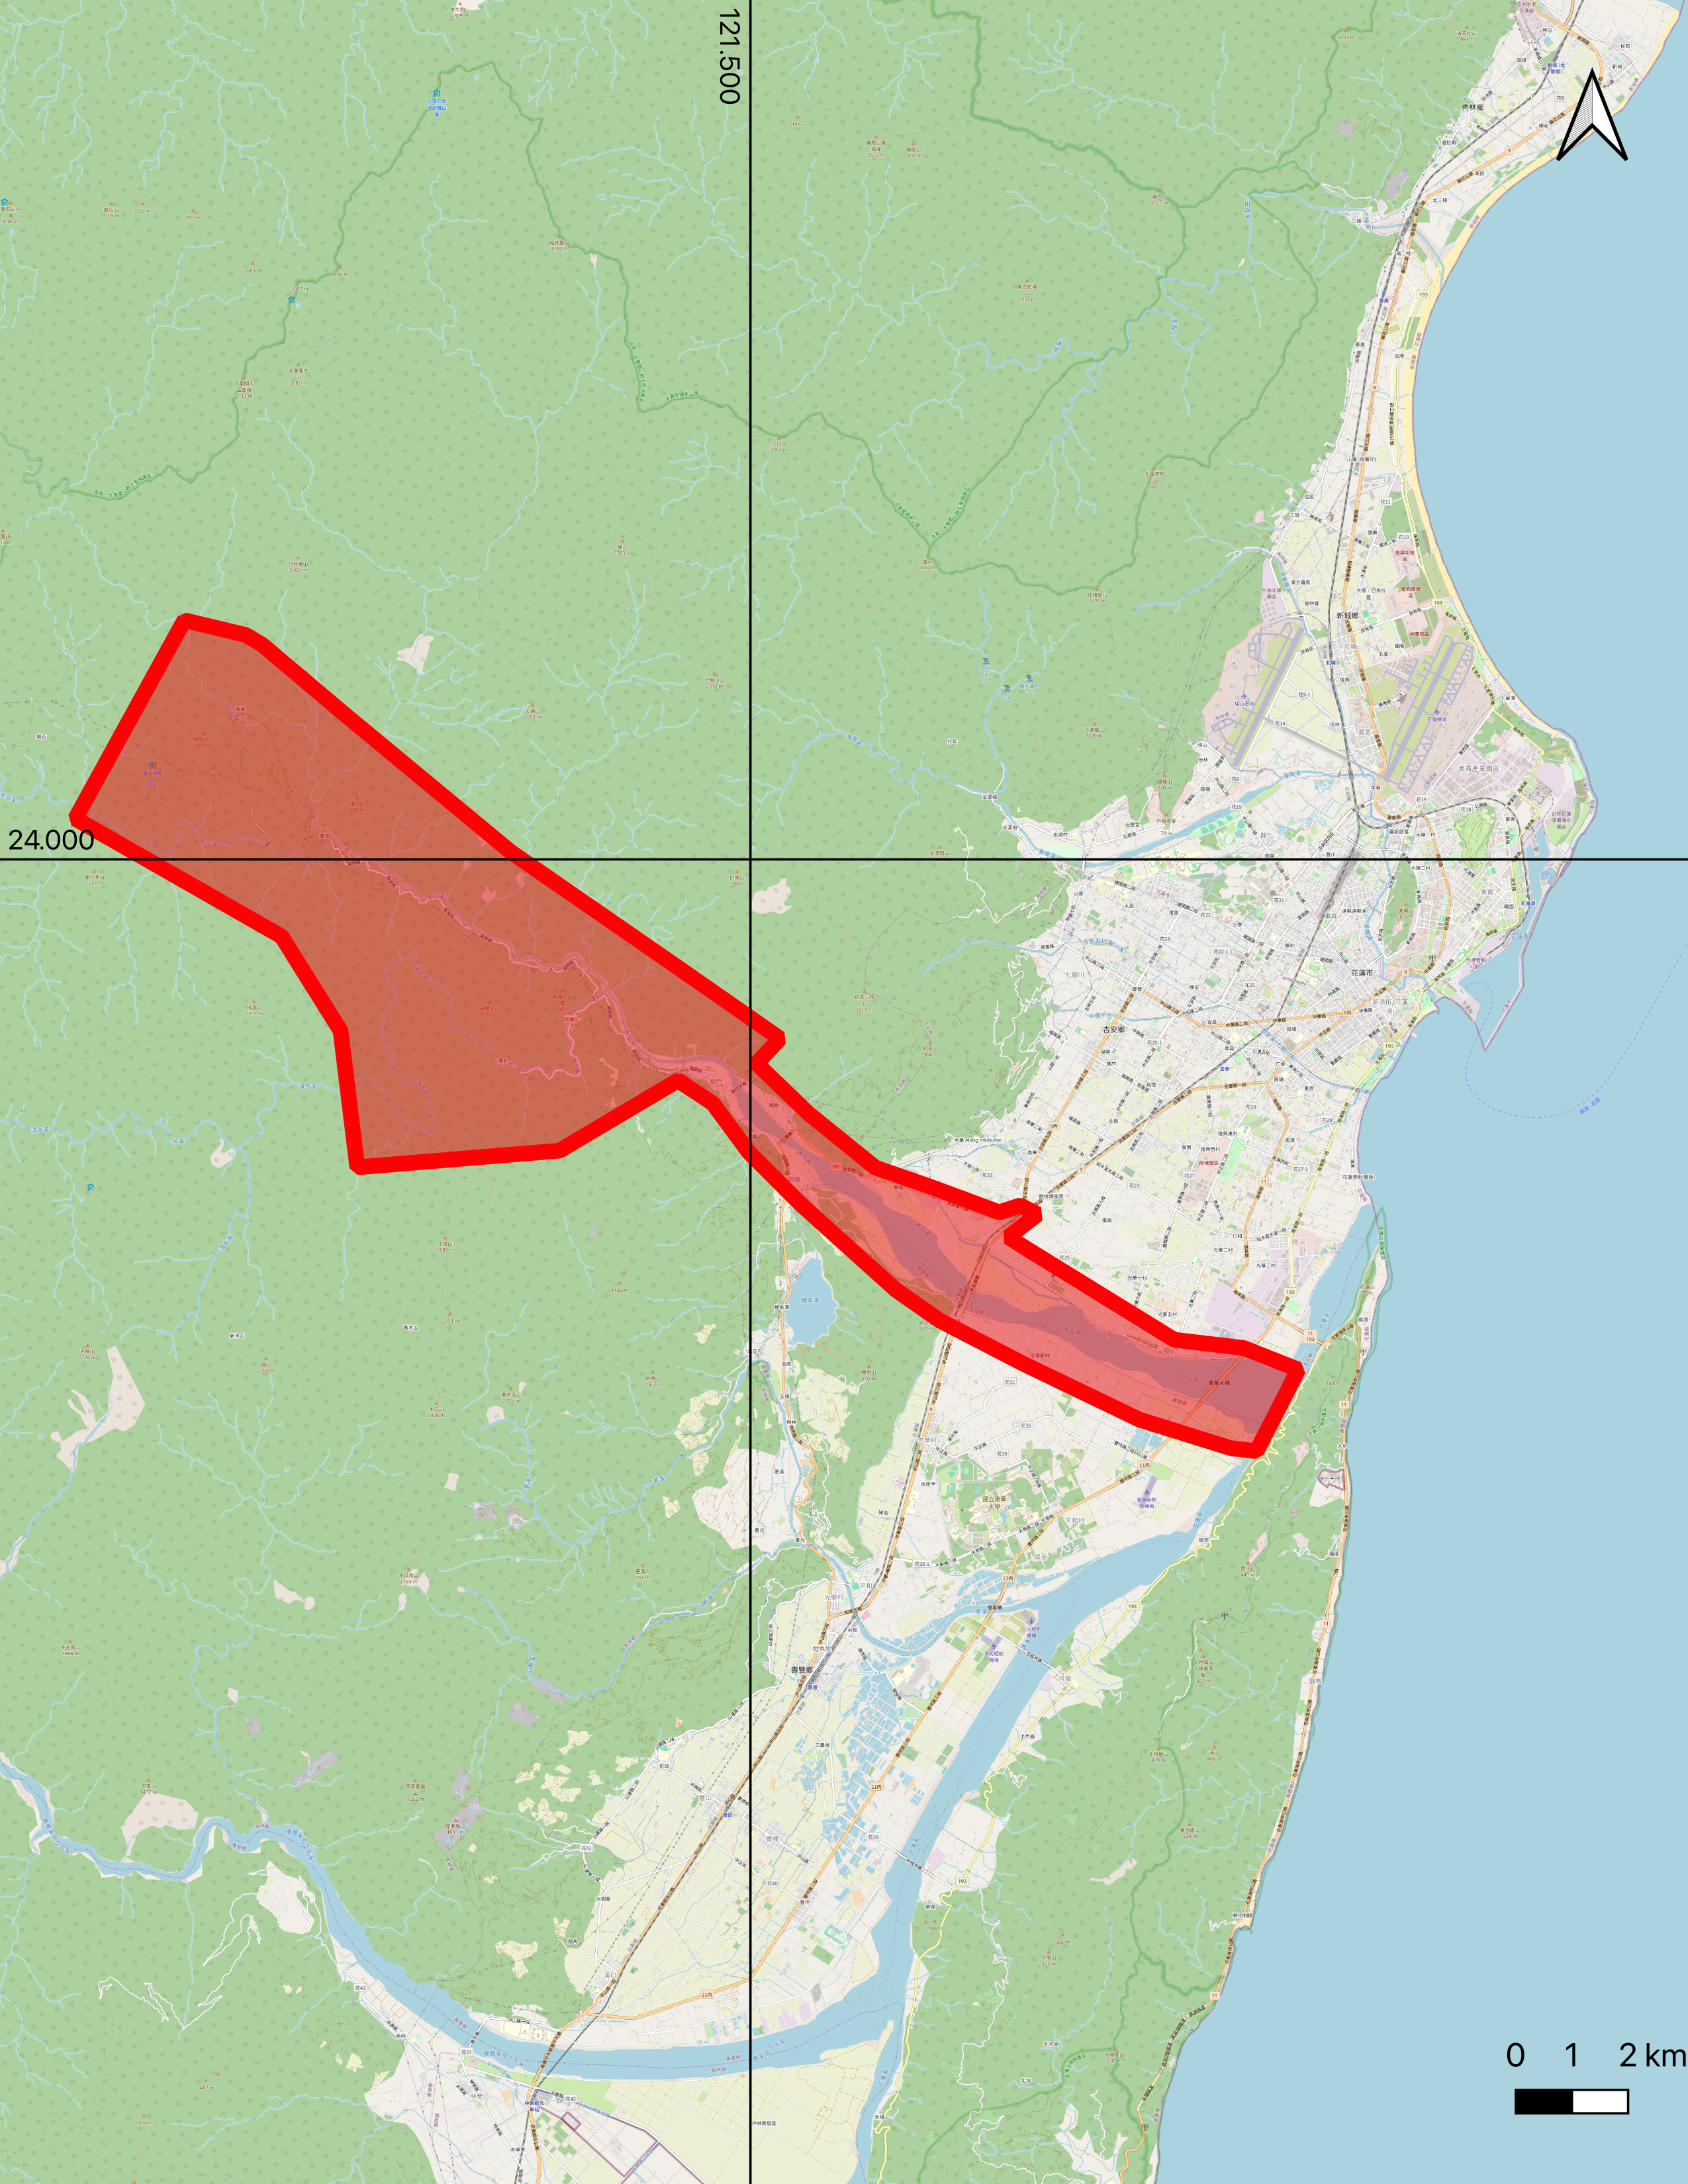
\includegraphics[width=0.95\linewidth]{figures/cases/case2_3.png} & 在花蓮縣壽豐鄉、吉安鄉和秀林鄉木瓜溪河畔* & 木瓜溪下游沿岸附近 & 位於花蓮縣壽豐鄉，靠近花蓮市南方約20公里，鄰近台9線與台11線交會處，接近花蓮溪河岸，位於農業區。\\ \hline
2-4 & & 在基隆河 & & \\ \hline
2-5 & & 在基隆河上游 & & \\ \hline
3-1 & 
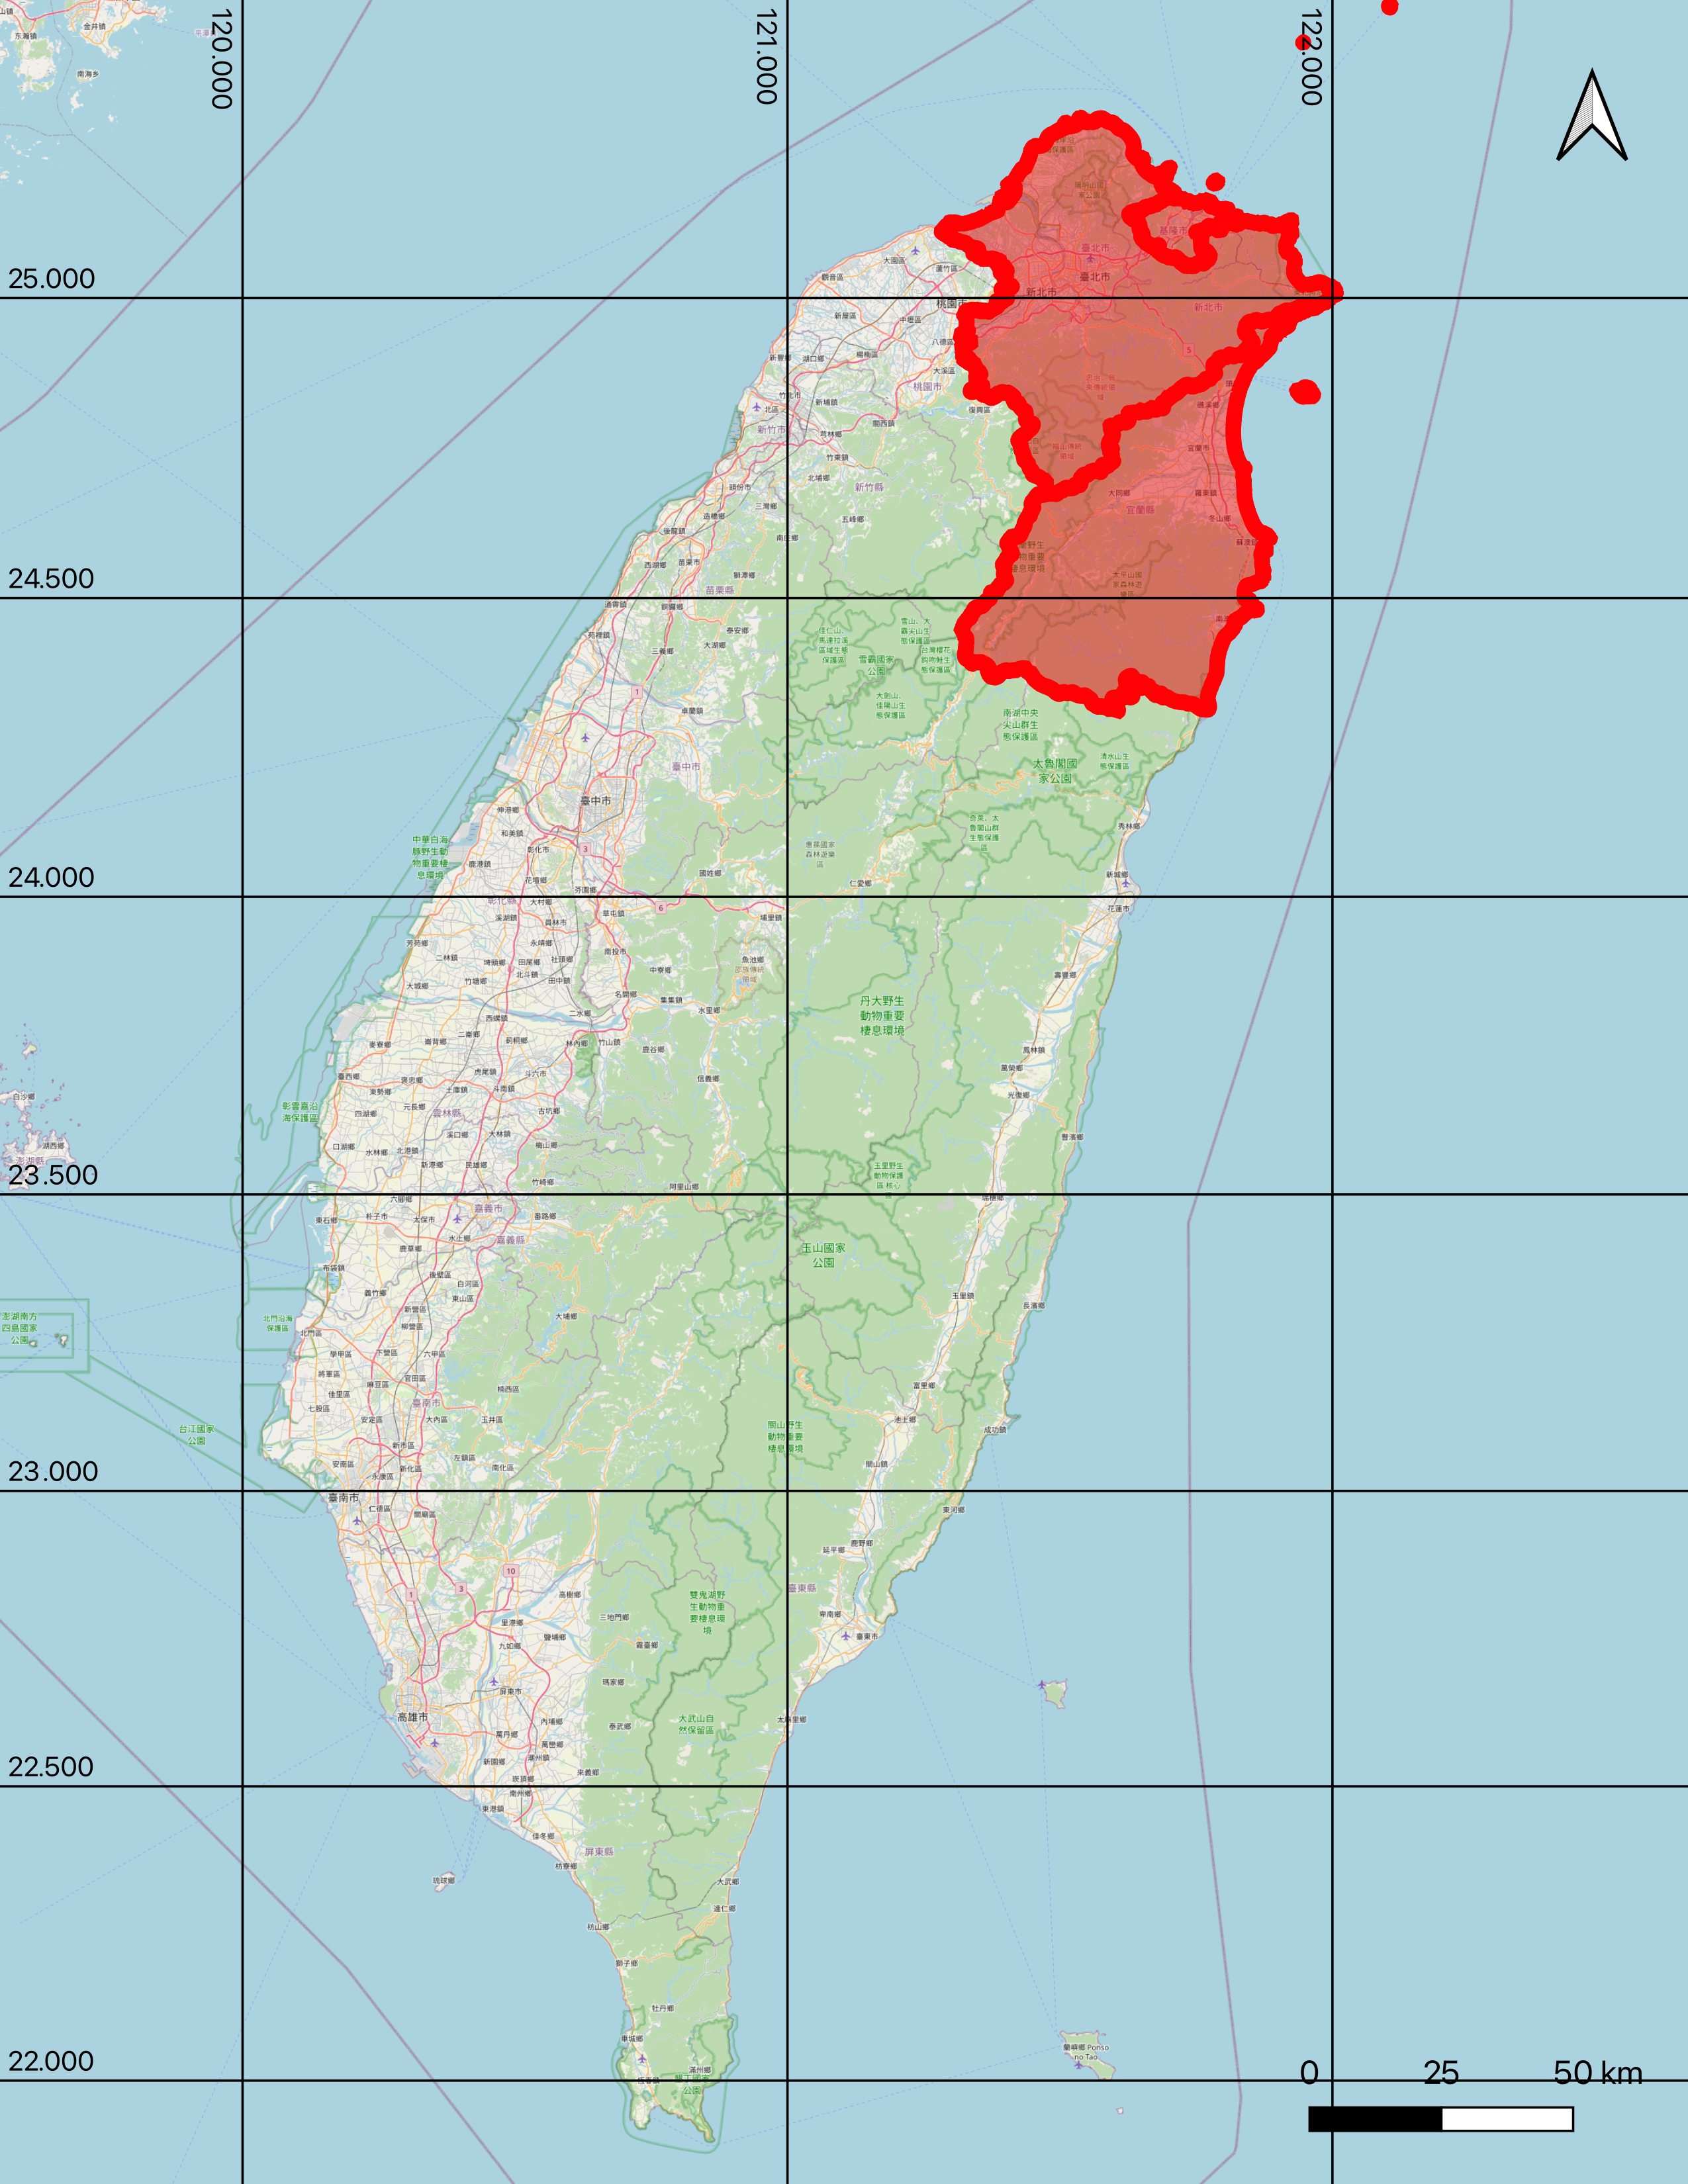
\includegraphics[width=0.95\linewidth]{figures/cases/case3_1.png} & 在台灣北部 & 東北地區 & 位於台北市東北部，靠近基隆市，鄰近基隆河岸，並接近台灣東北角海岸，主要道路如基隆路和中山高速公路交會處，周圍為住宅區和商業區混合地帶。 \\ \hline
3-2 &
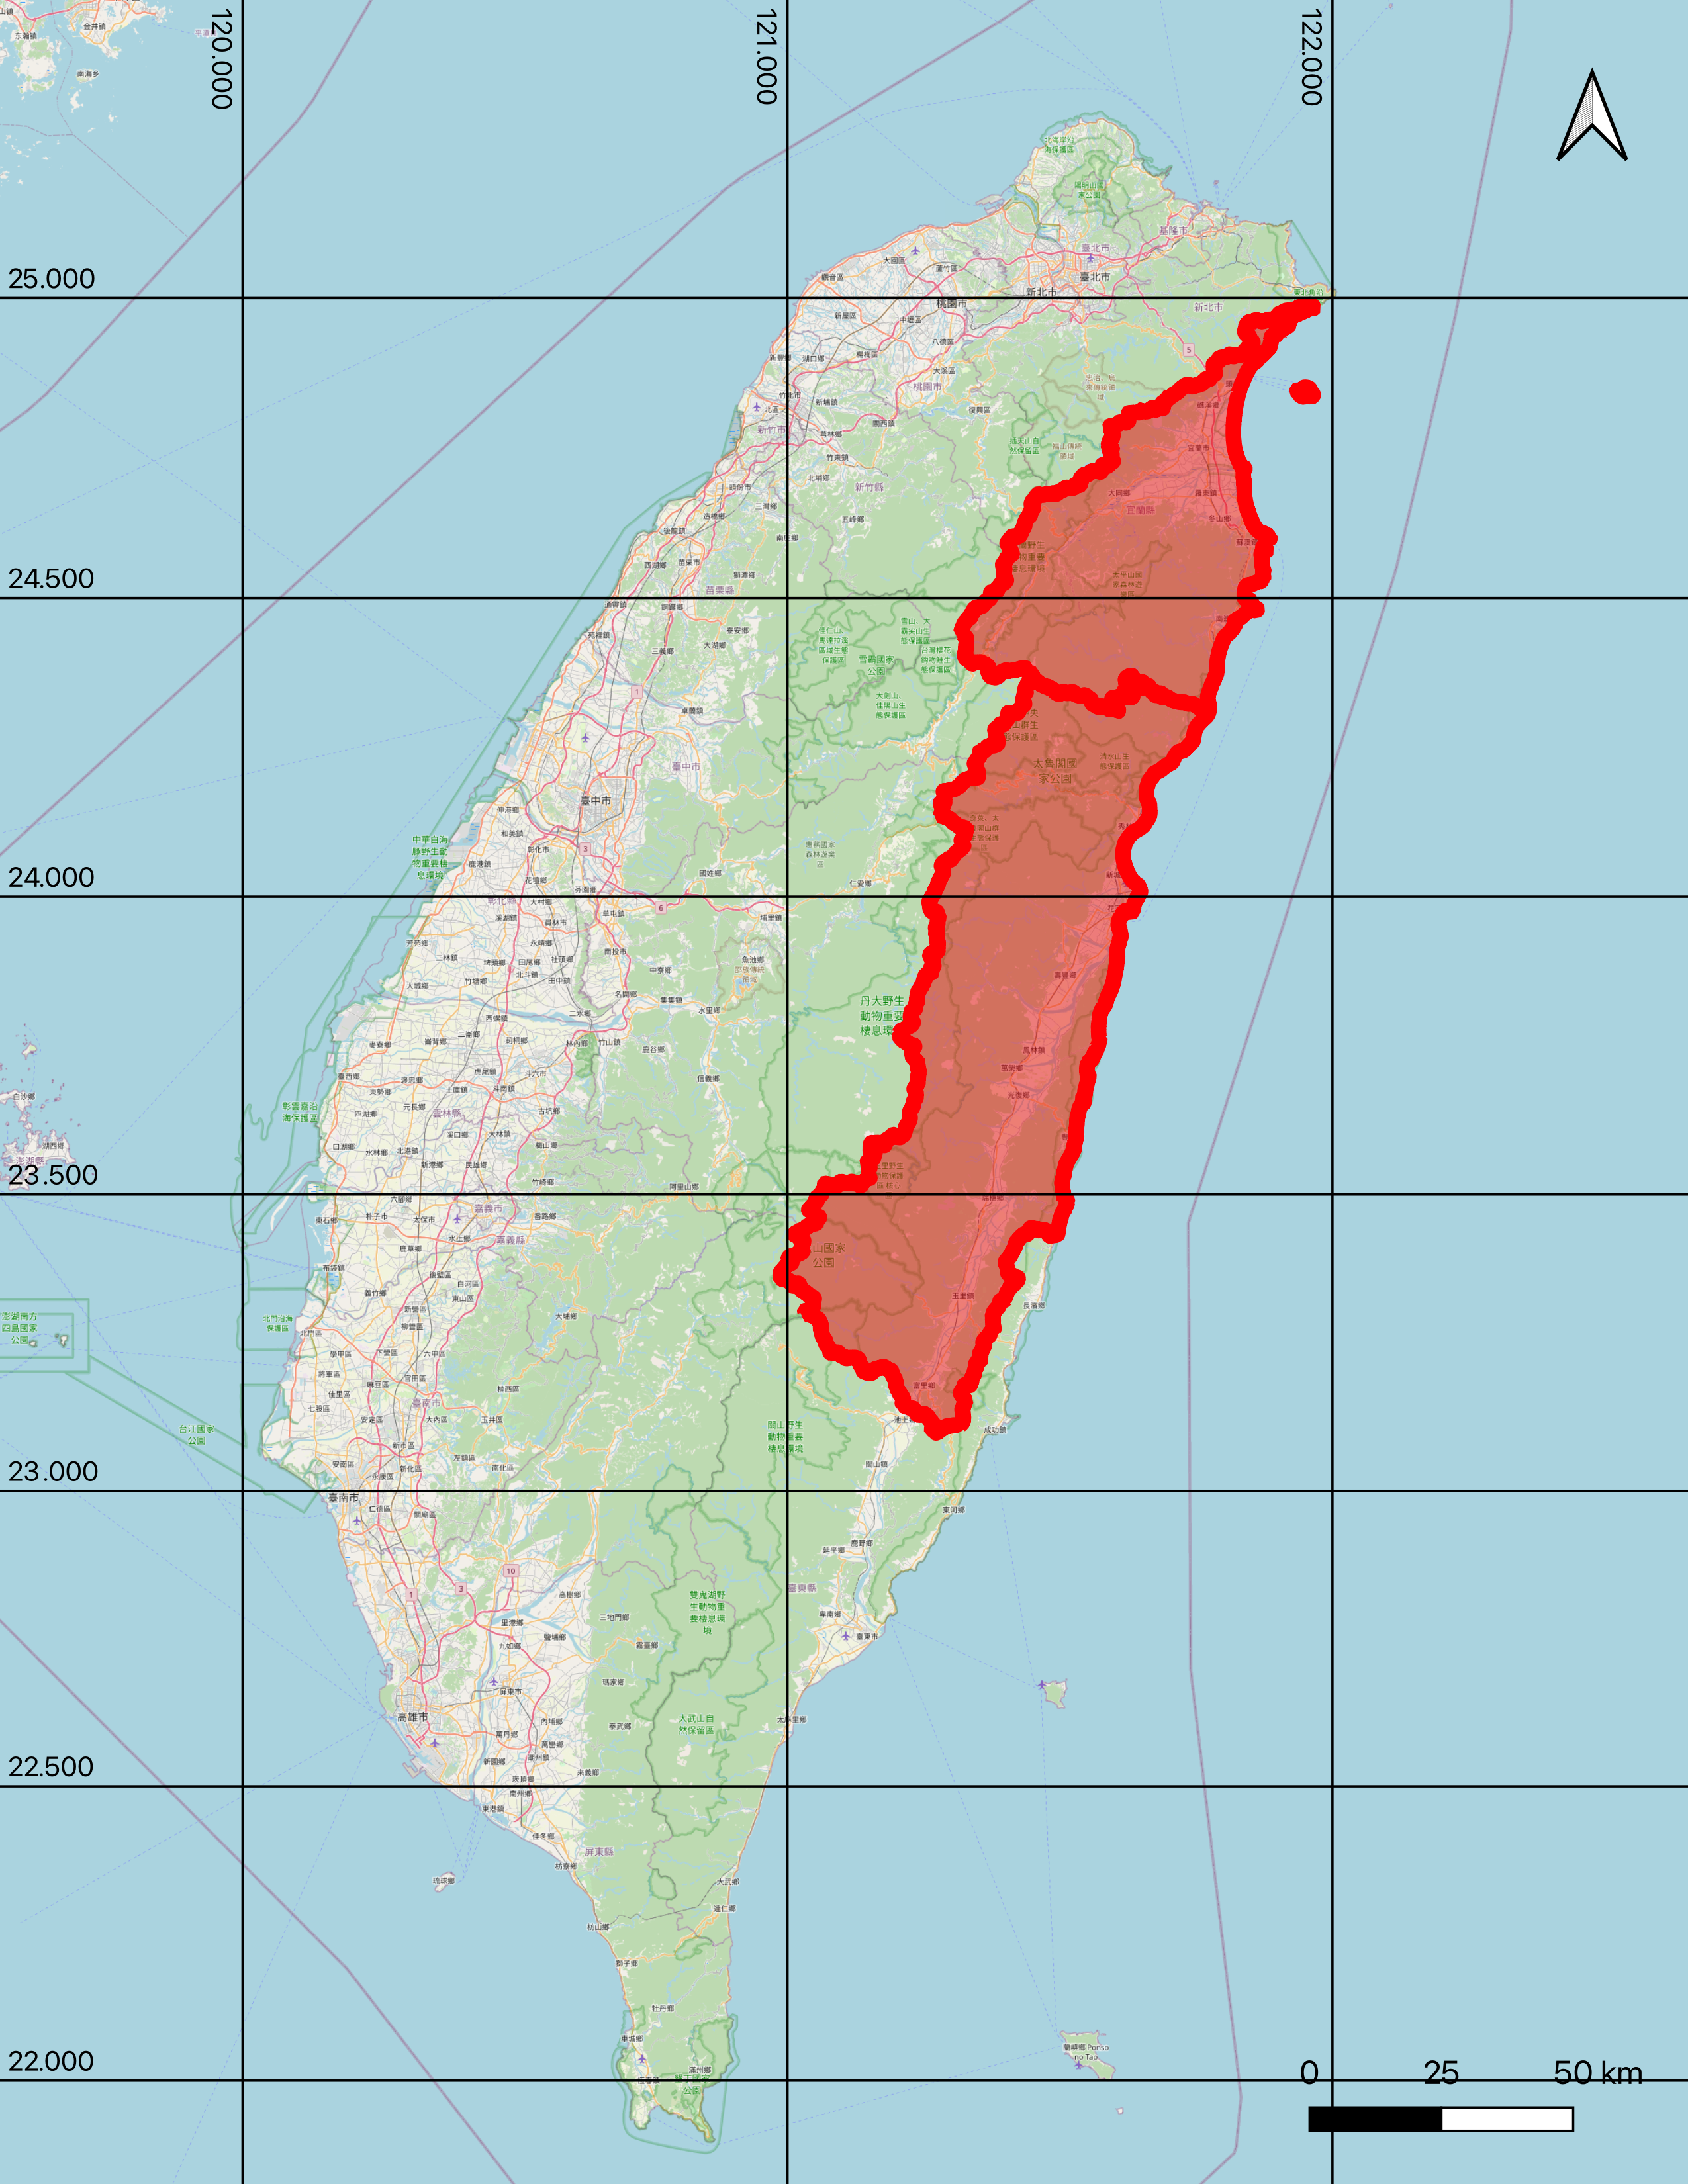
\includegraphics[width=0.95\linewidth]{figures/cases/case3_2.png} & 在台灣東北部 & 花蓮地區 & 位於宜蘭縣東北部海域，鄰近蘇澳鎮，靠近台灣東北海岸，距離台北市約100公里，周圍為海洋環境，無明顯陸地地標。 \\ \hline
3-3 &
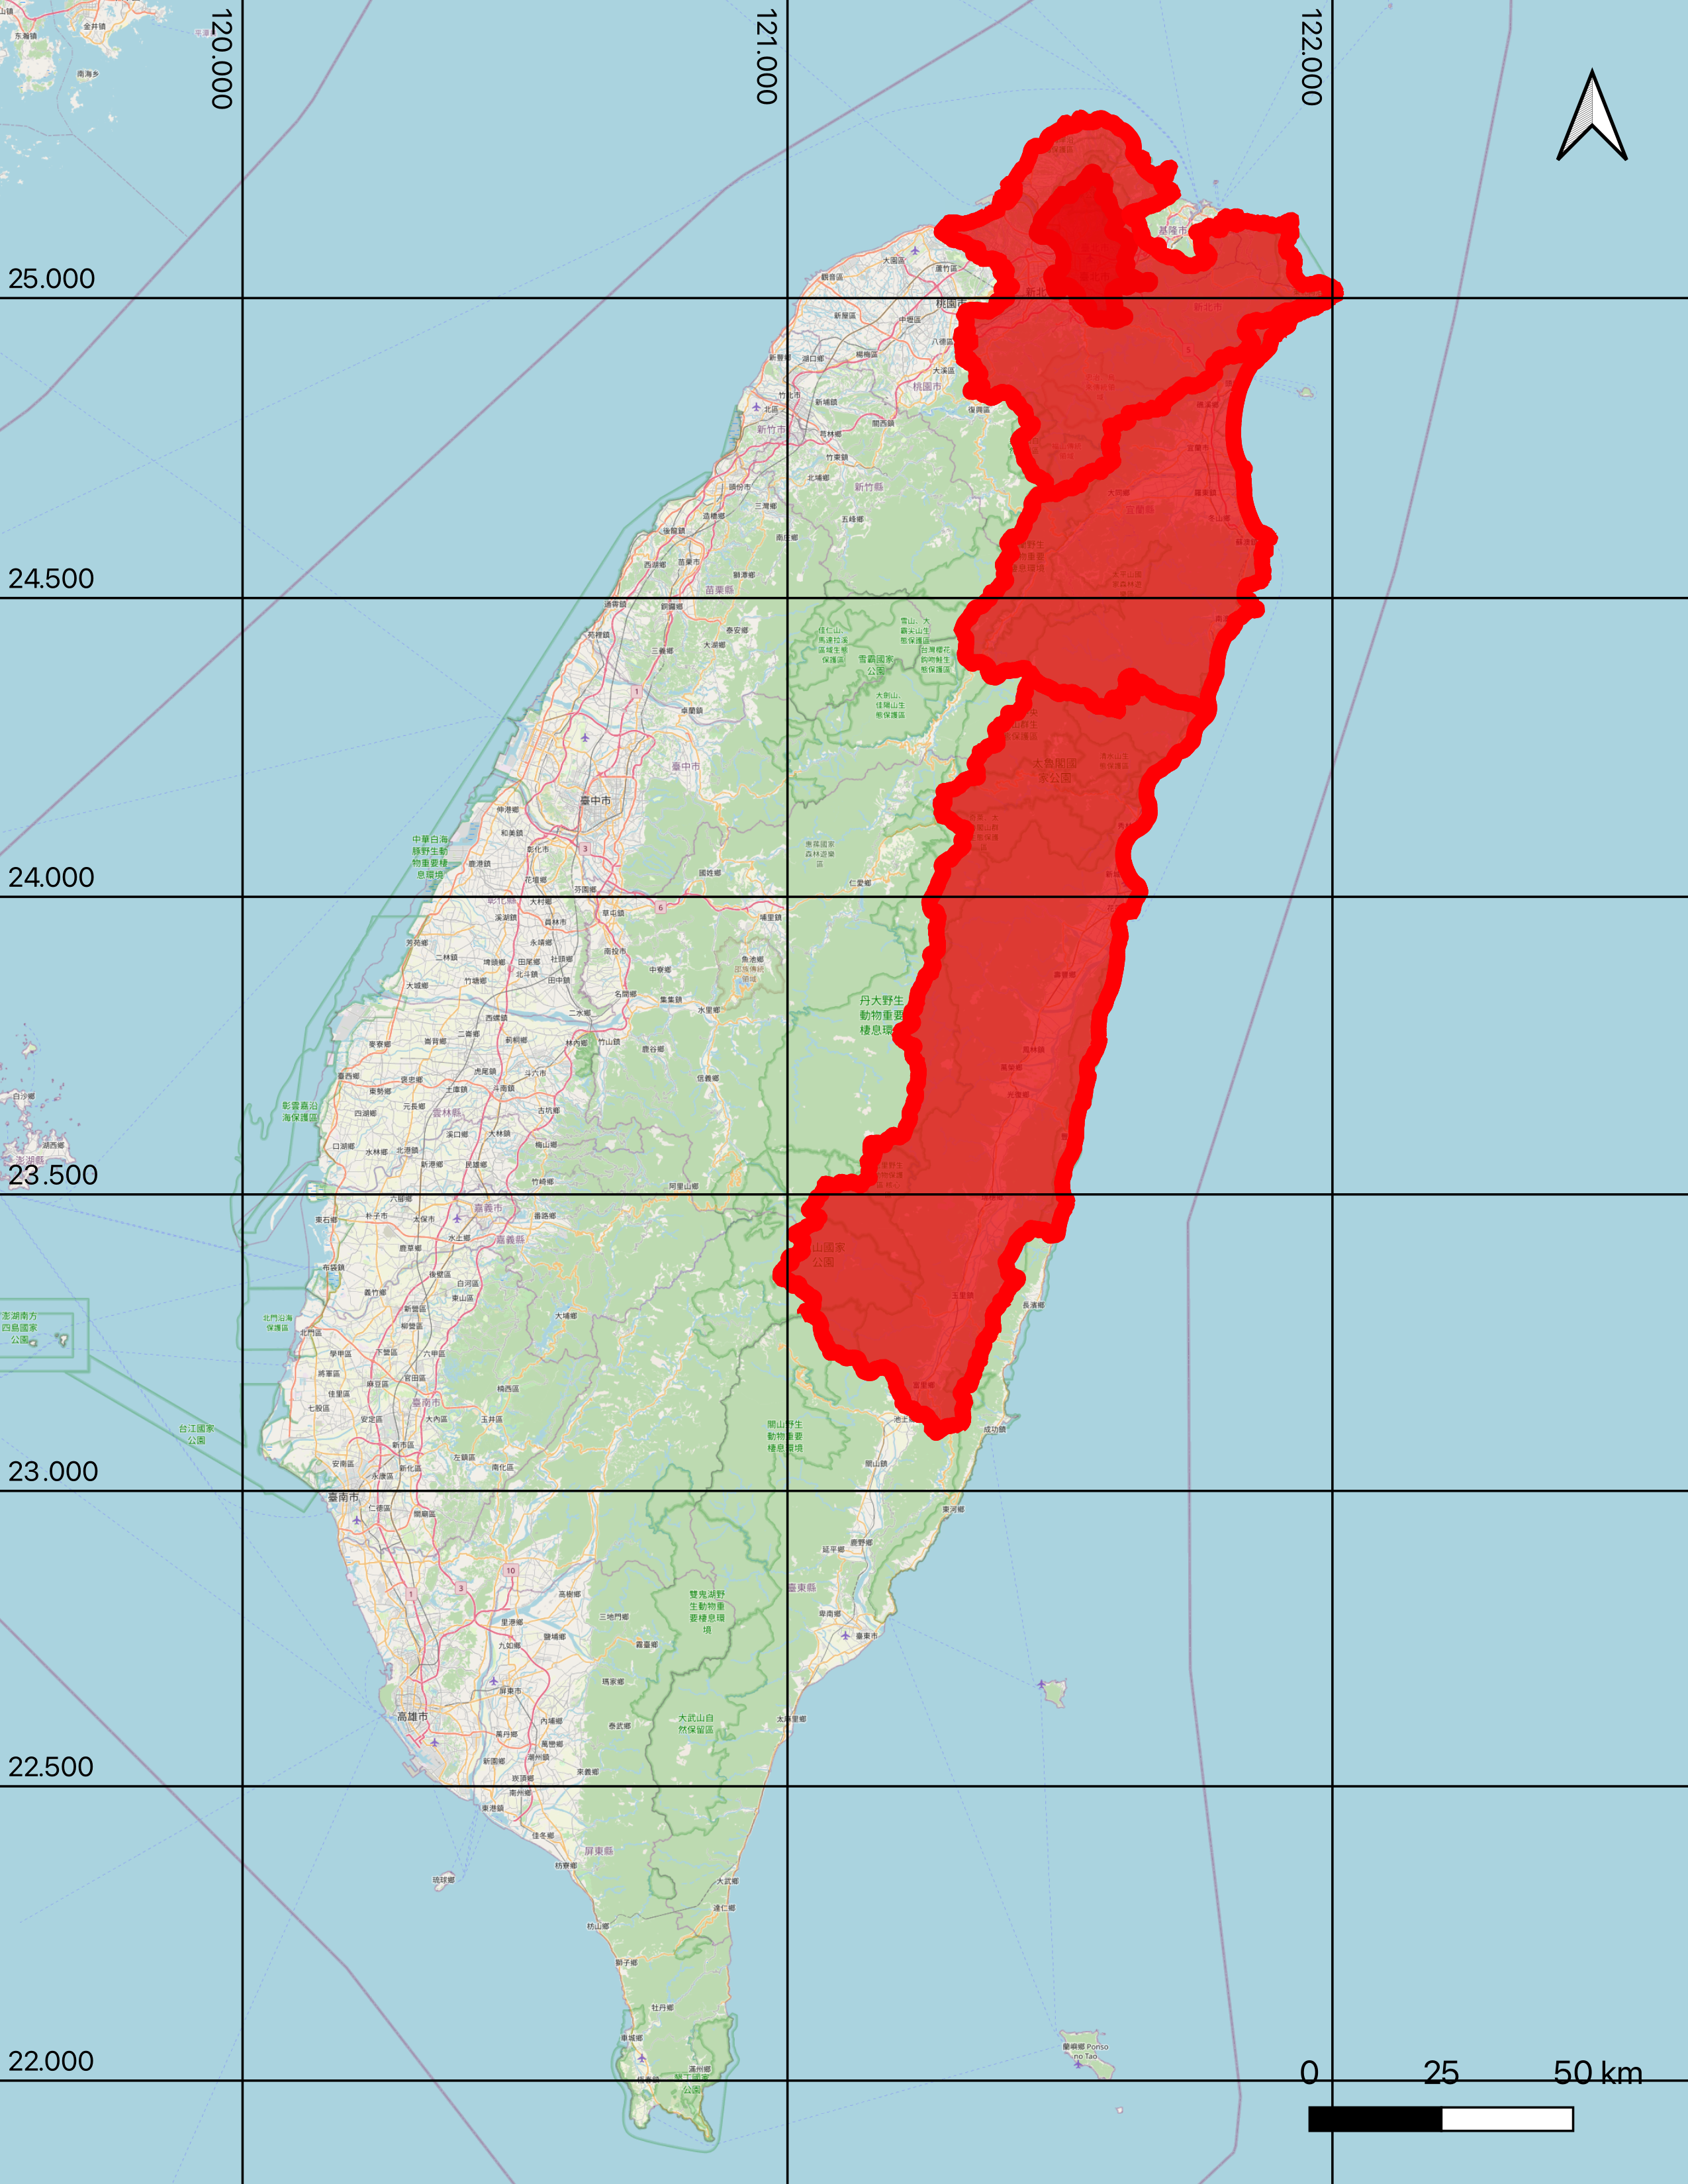
\includegraphics[width=0.95\linewidth]{figures/cases/case3_3.png} & 在台灣沿岸* & 東北地區 & 主要影響範圍包括台北市中山區，靠近台北101西南約500公尺，並延伸至新北市淡水河岸，涵蓋台灣東北部地區，部分影響範圍達至宜蘭縣及花蓮縣沿海地區。 \\ \hline
3-4 & & 位於宜蘭縣近海 & & \\ \hline
3-5 & & 位於臺灣東部海域 & & \\ \hline
3=6 & & 位於花蓮縣壽豐鄉 & & \\ \hline
4-1 &
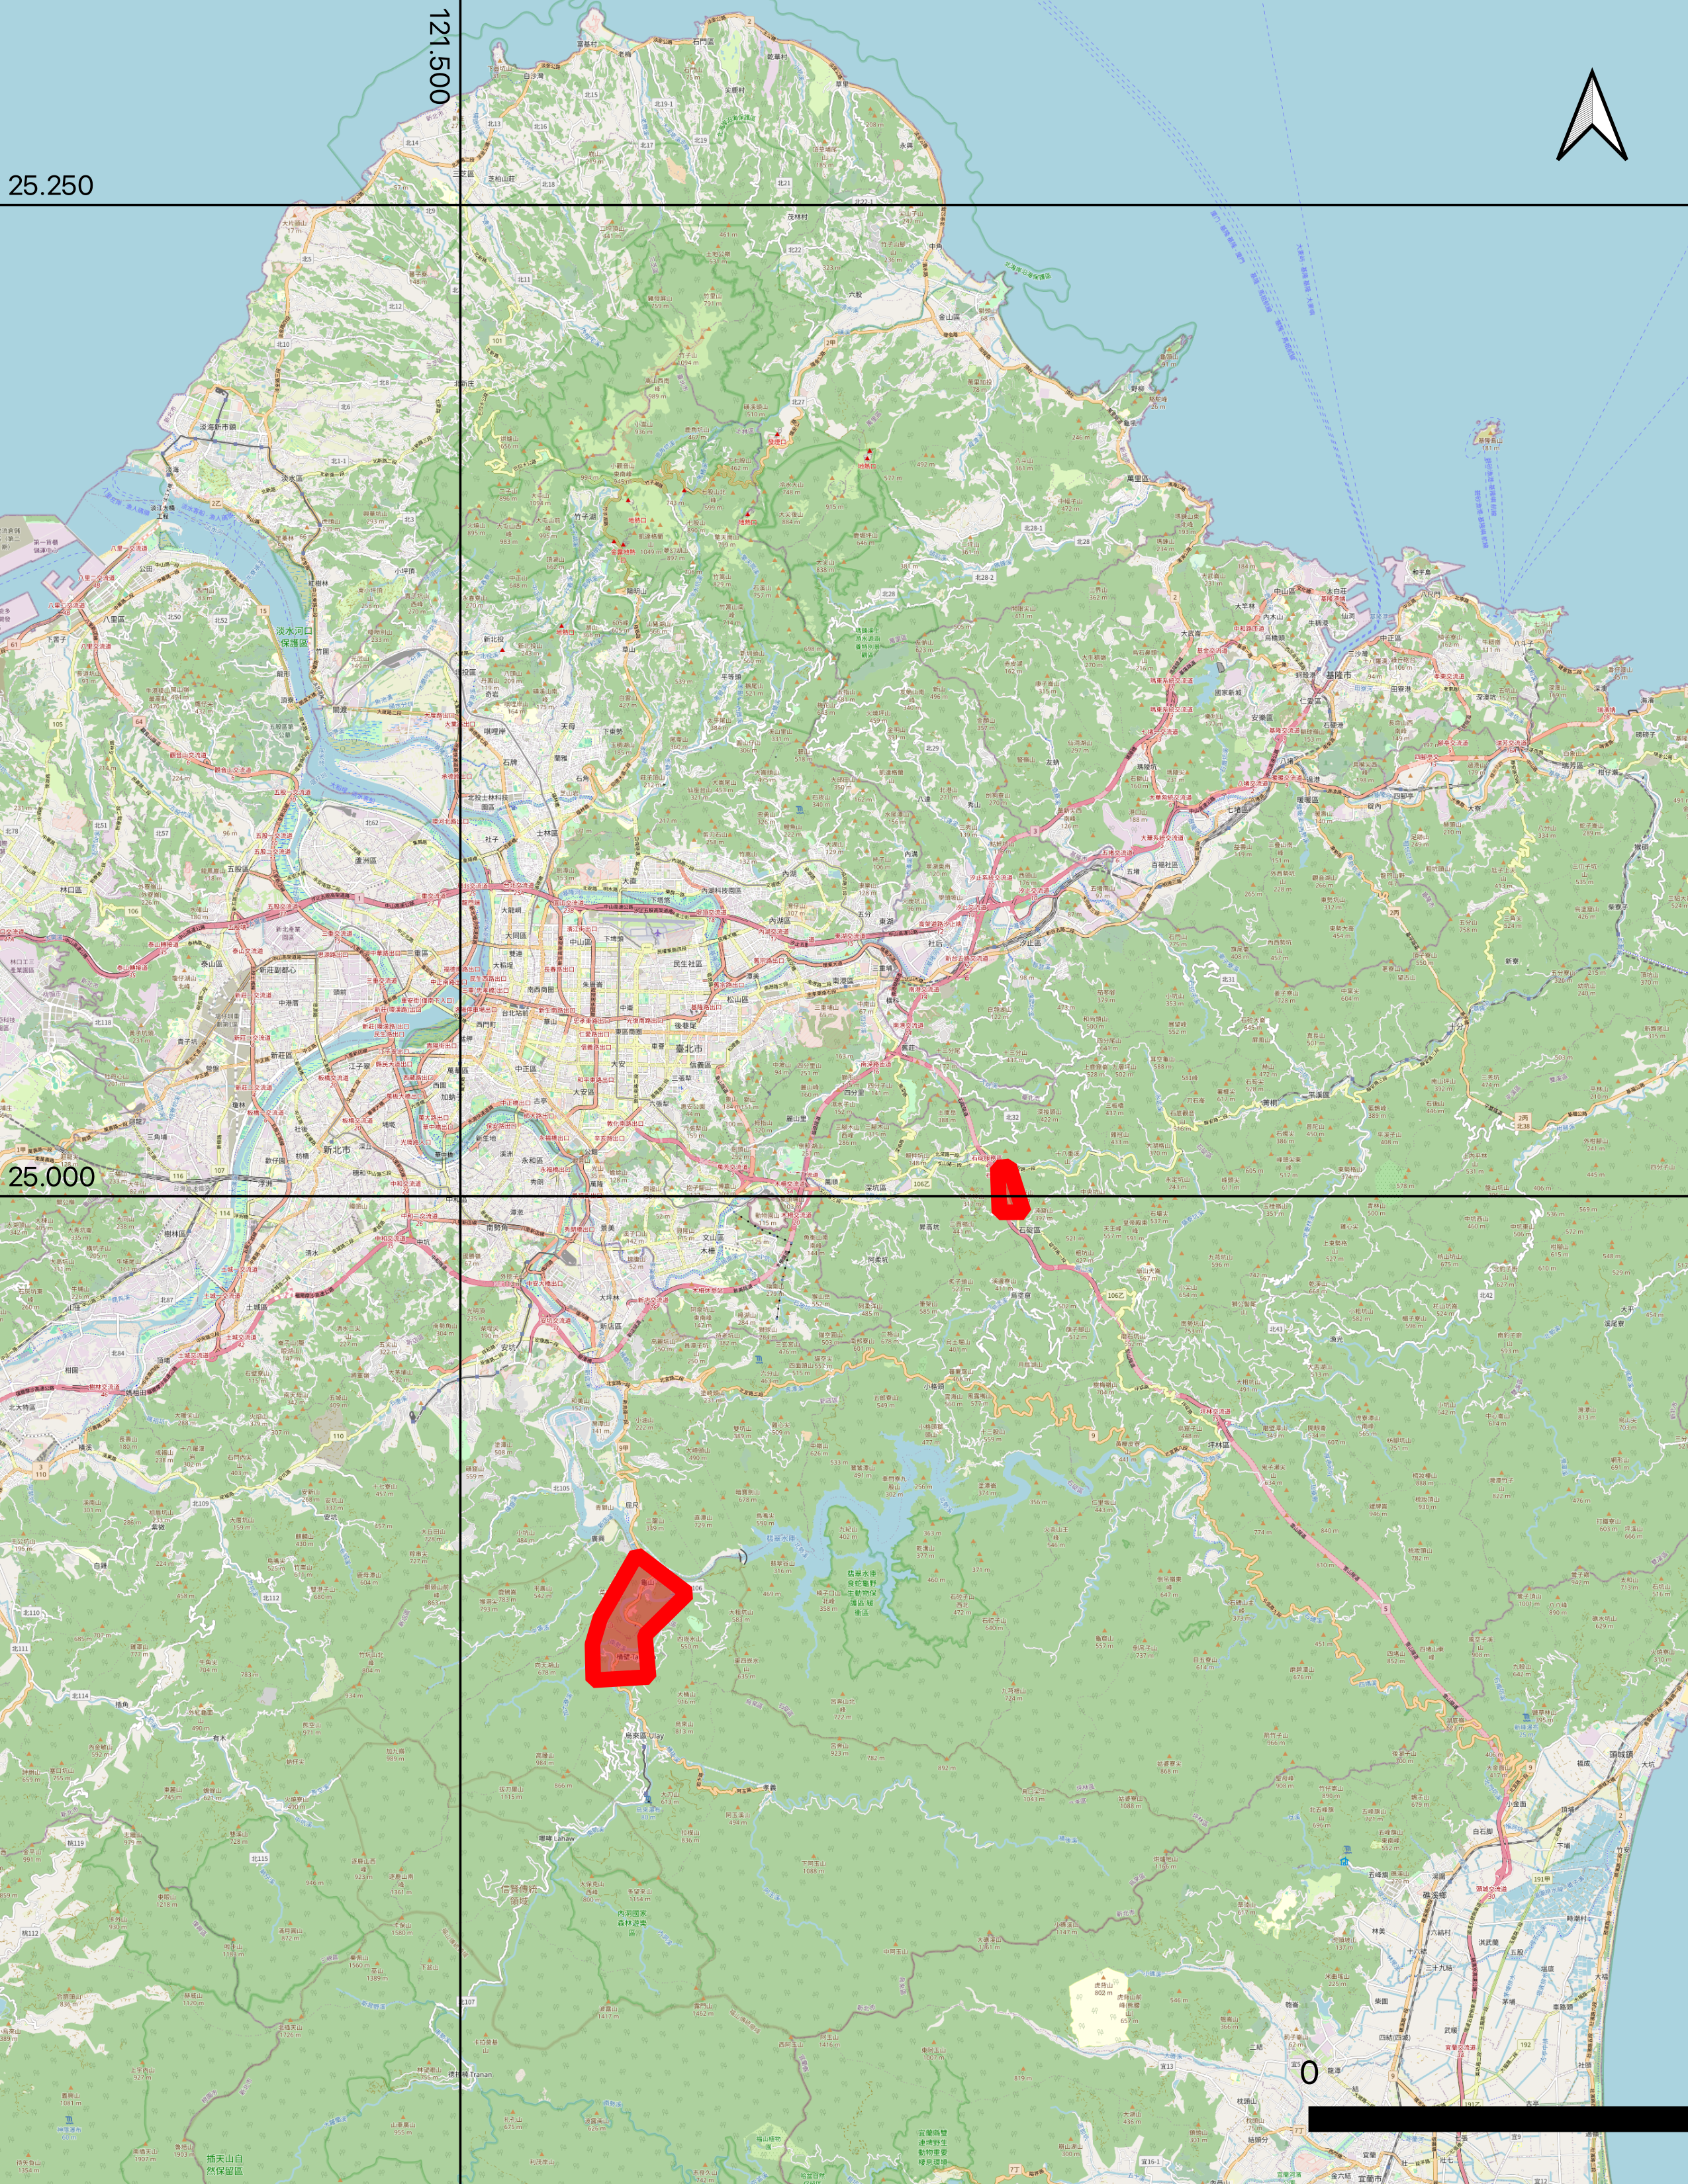
\includegraphics[width=0.95\linewidth]{figures/cases/case4_1.png} & 在新北市烏來區和新店區（新店溪河畔）& 您所在區域附近 & 位於新北市汐止區，靠近汐止火車站東南約1公里，鄰近台5線與台62線交會處，周圍為住宅區，靠近基隆河岸。／位於台北市內湖區，鄰近內湖科技園區，靠近成功路與民權東路交會處，周圍為商業區，靠近基隆河岸。 \\ \hline
4-2 &
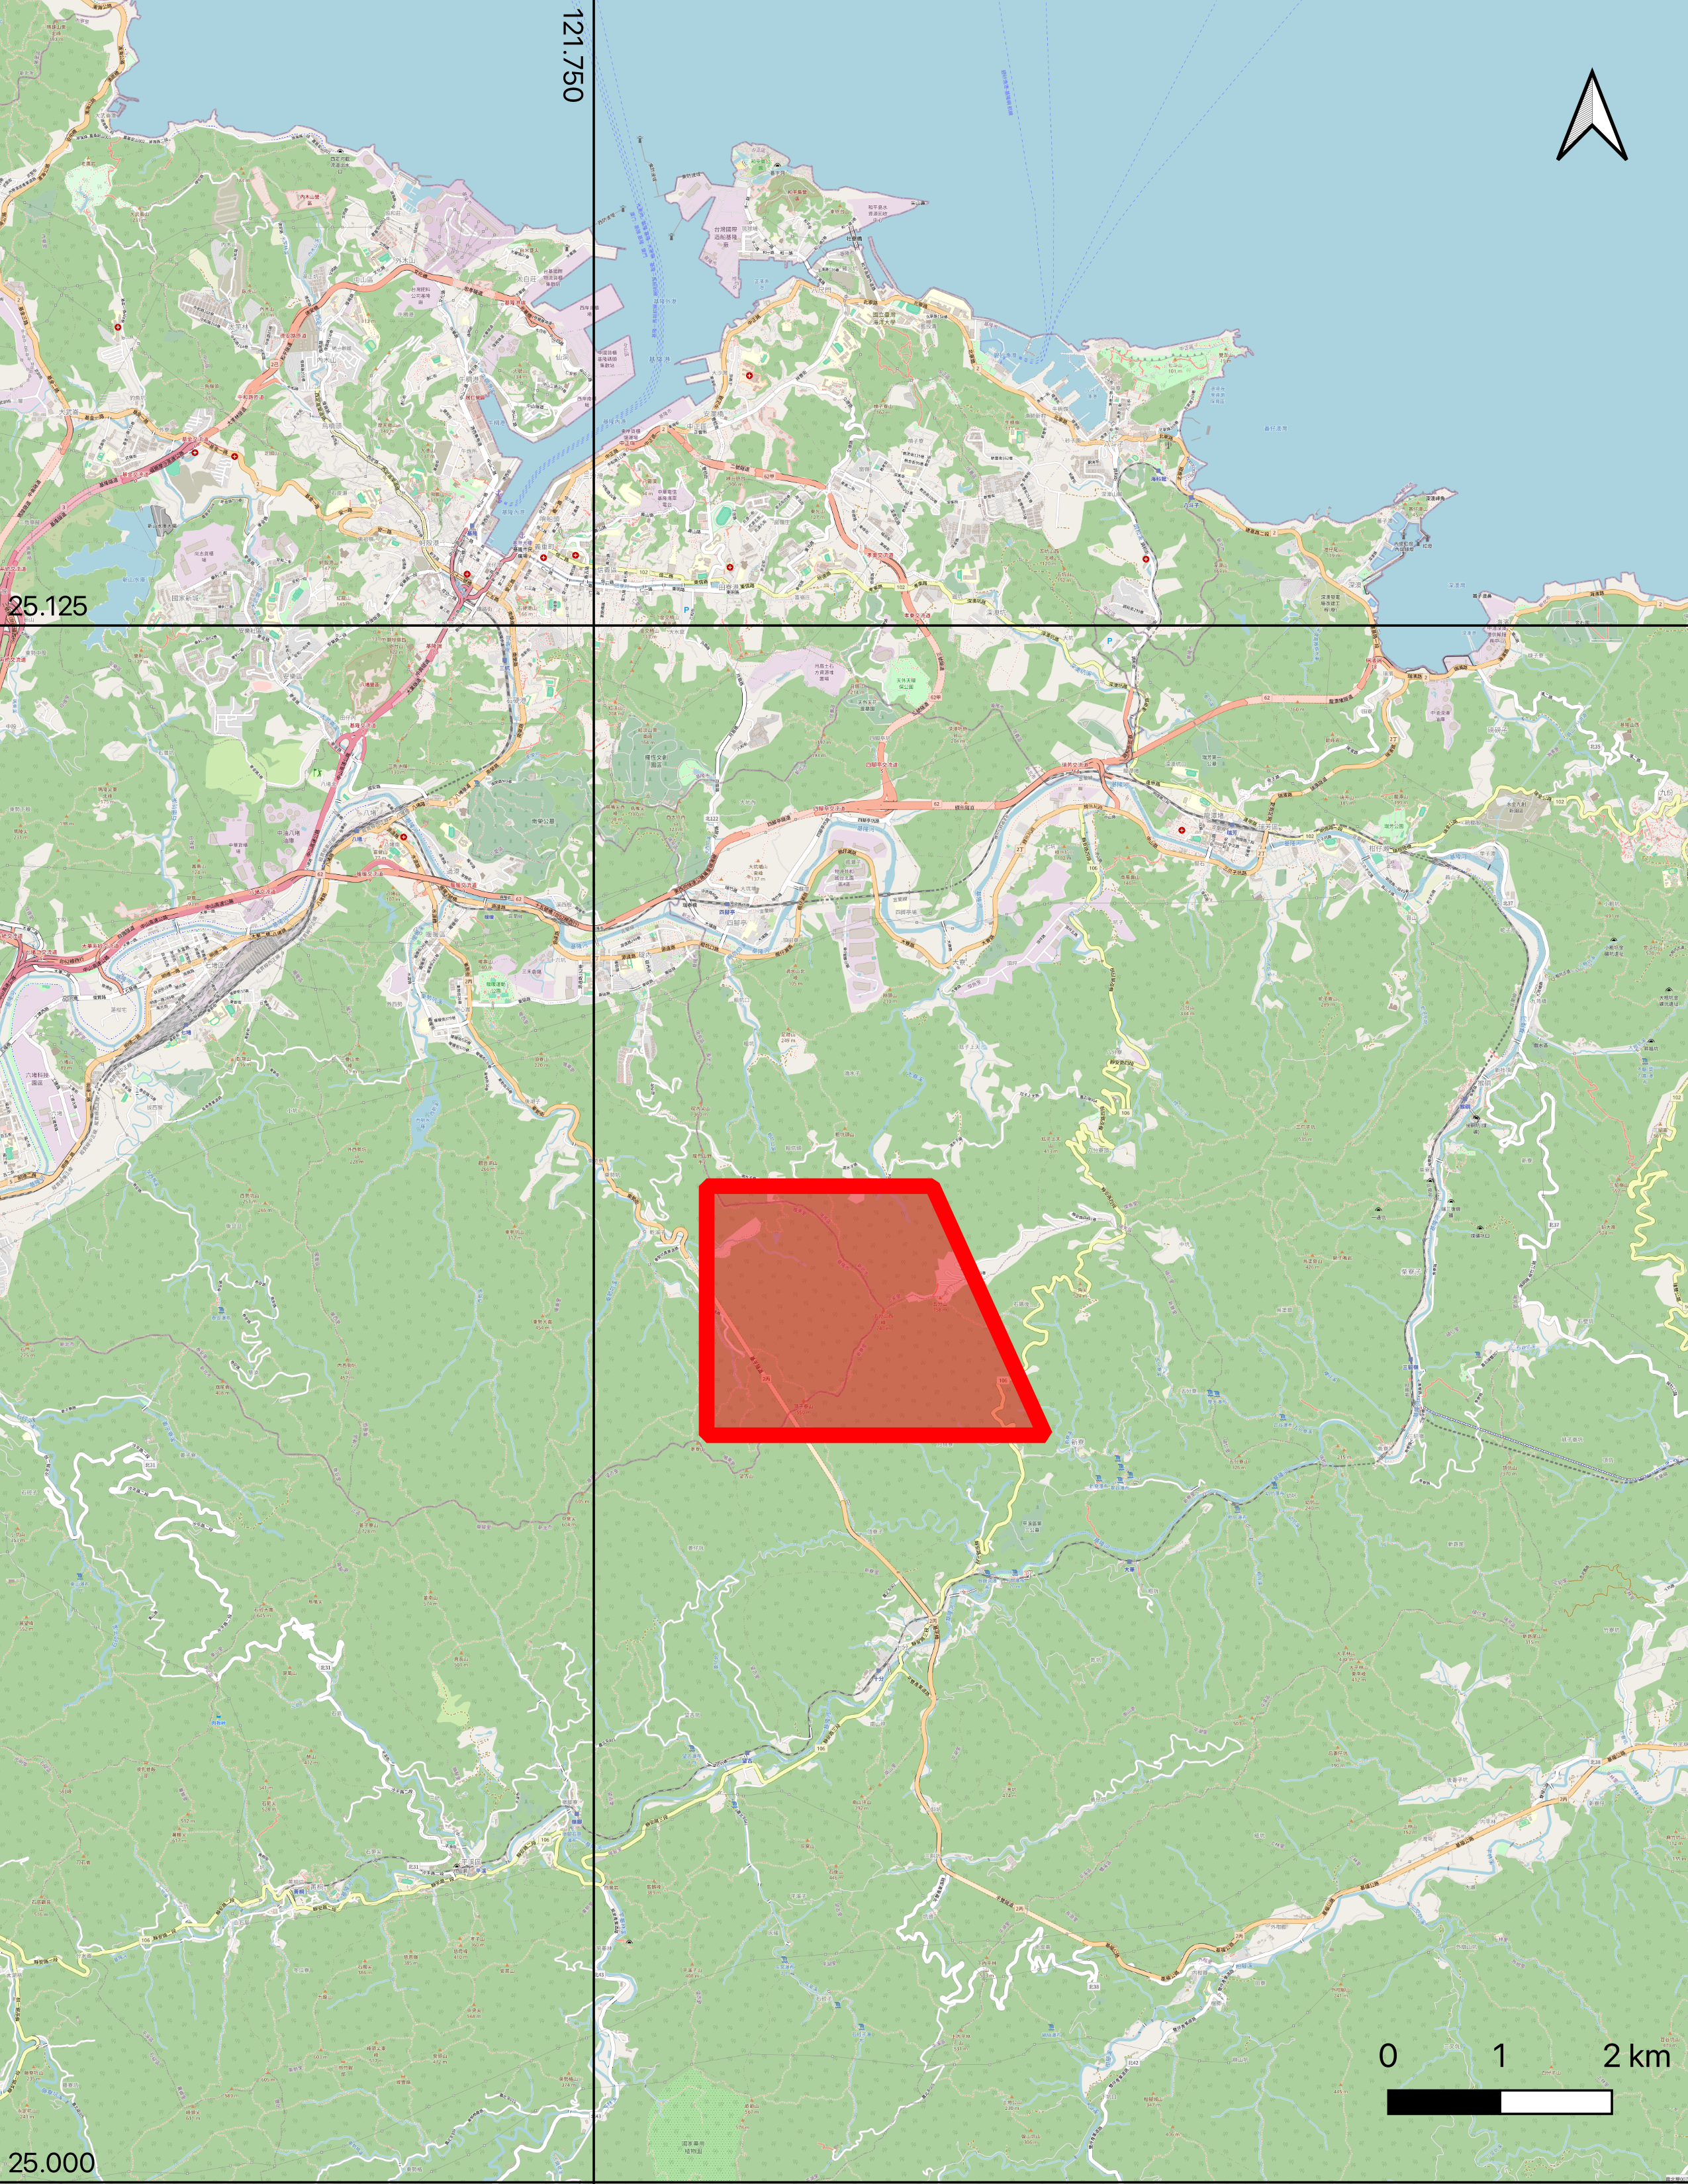
\includegraphics[width=0.95\linewidth]{figures/cases/case4_2.png}  & 在基隆市暖暖區、新北市平溪區和新北市瑞芳區(五分山) & 您所在區域附近 & 位於台北市內湖區，靠近基隆河岸，鄰近台北101東北約4公里，位於成功路和民權東路交會處，屬於商業區。 \\ \hline
4-3 &
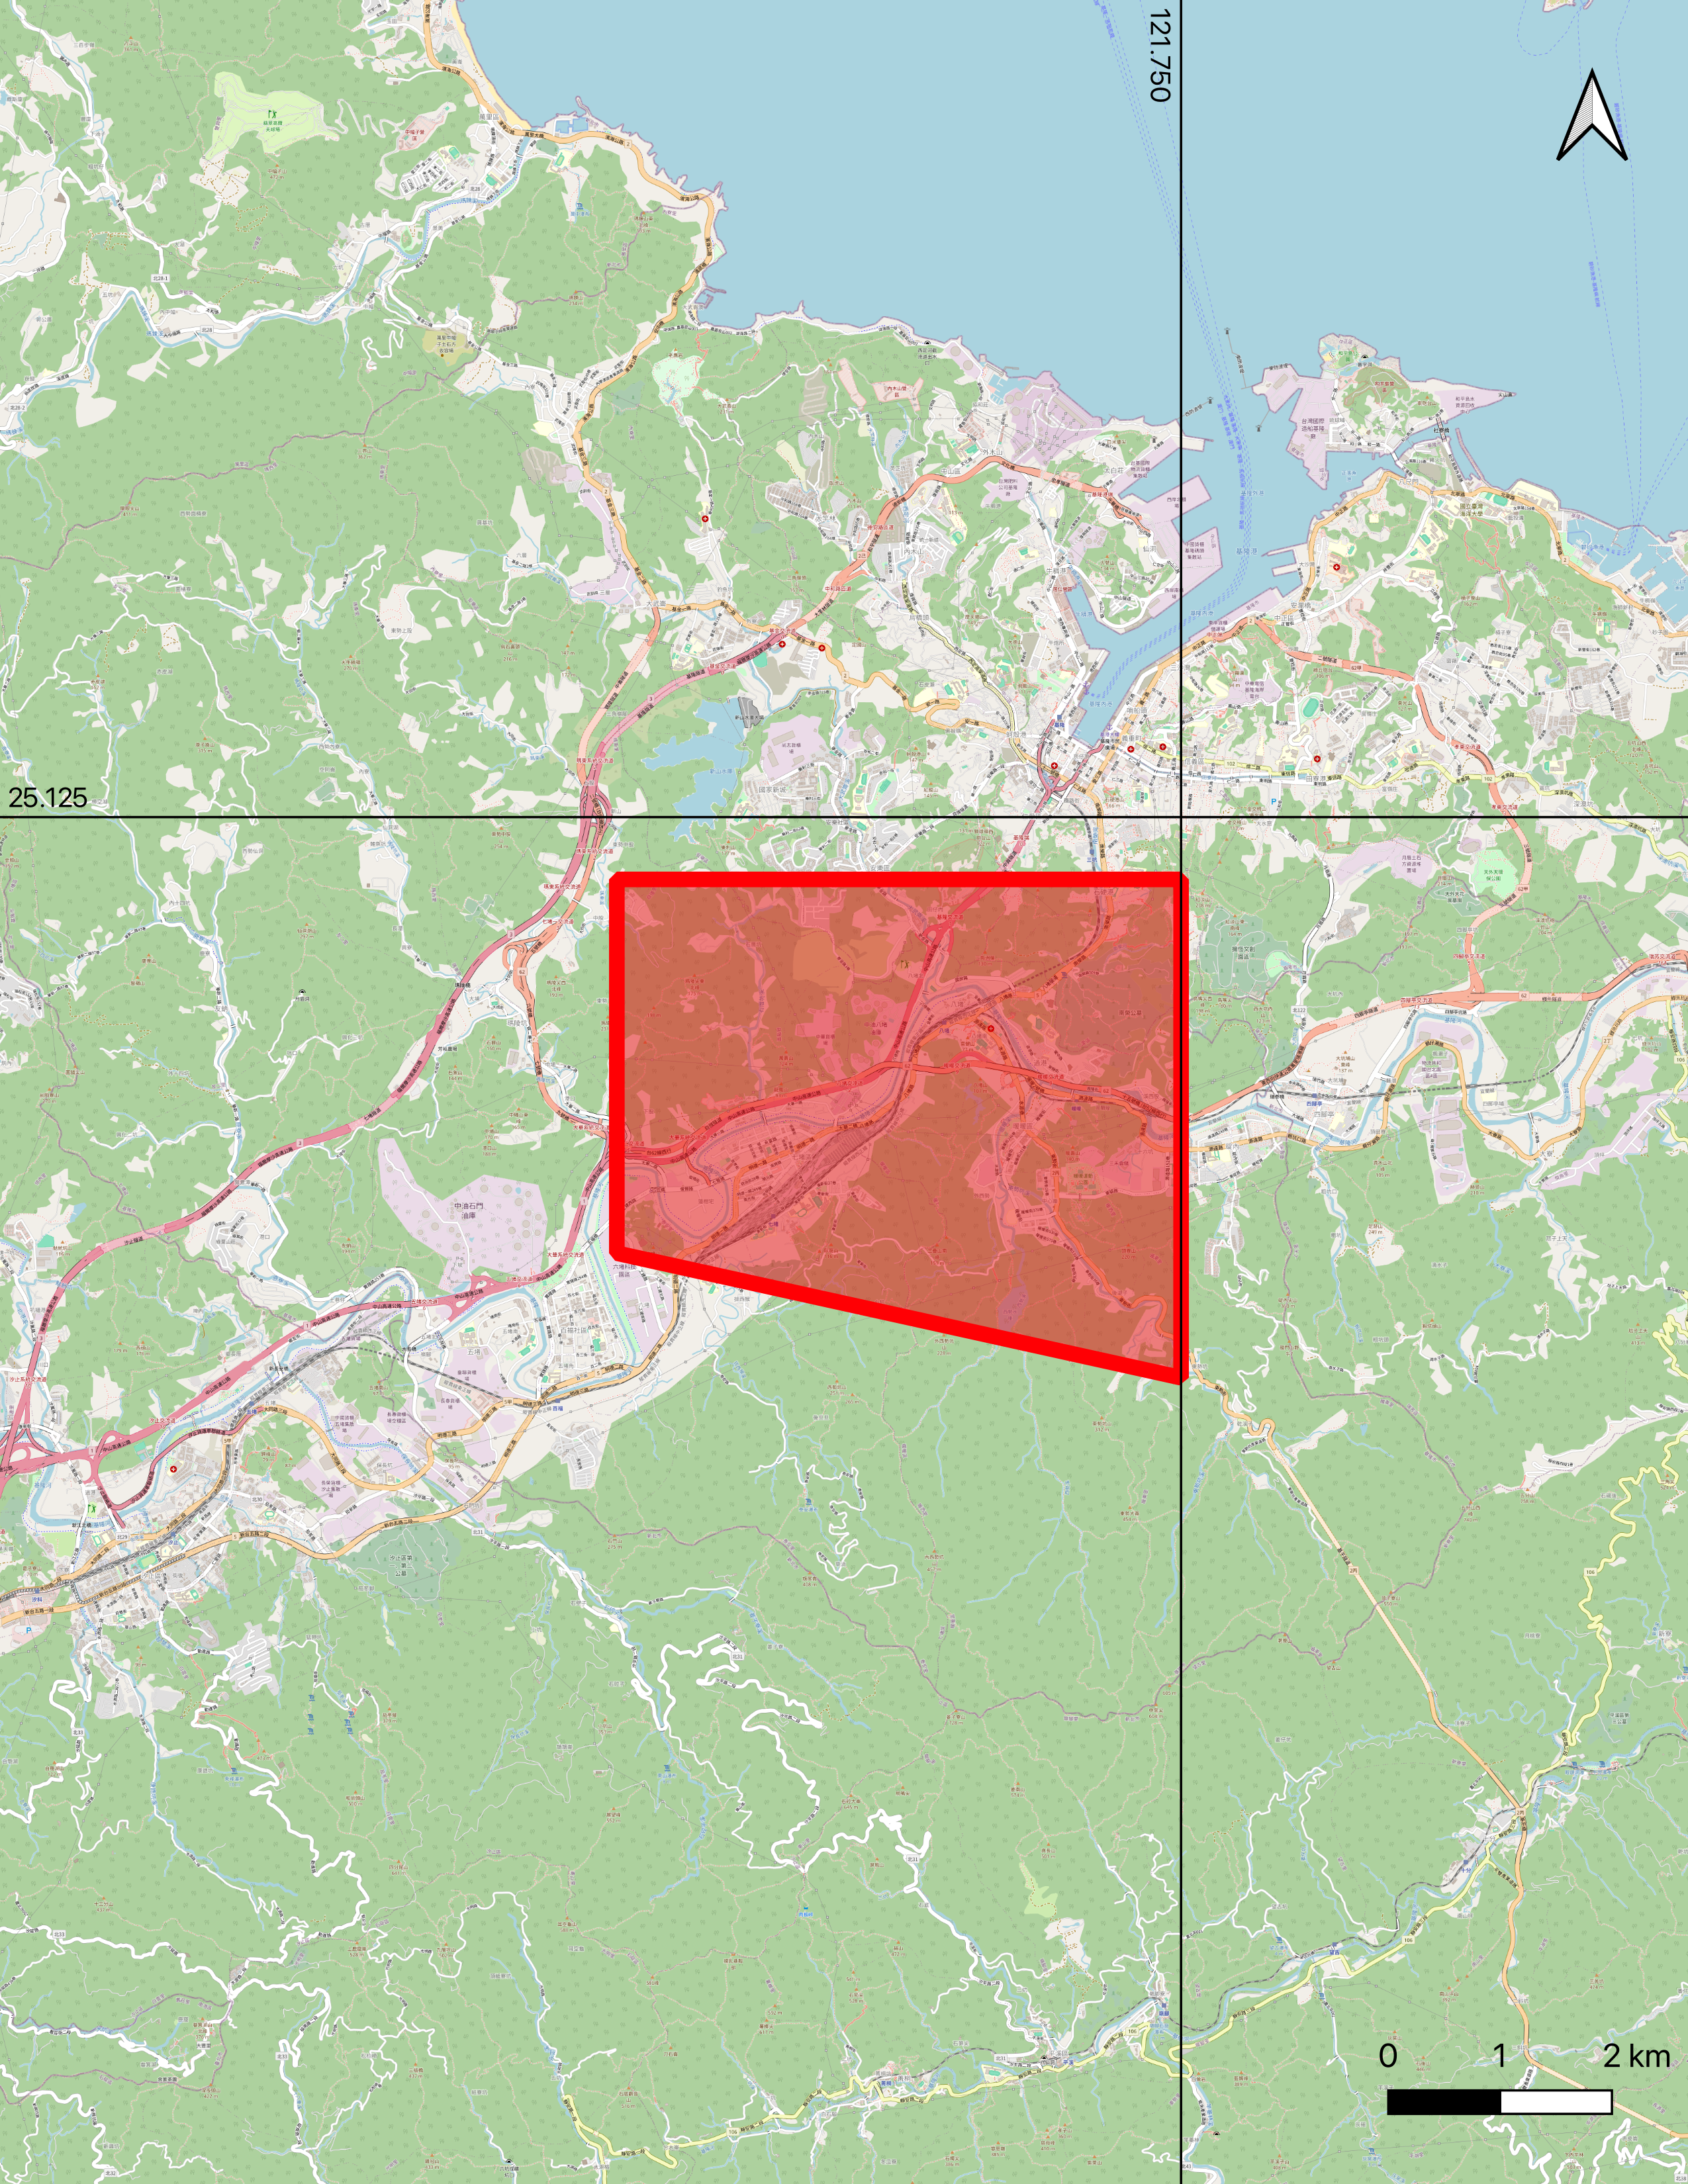
\includegraphics[width=0.95\linewidth]{figures/cases/case4_3.png} & 在基隆市暖暖區、新北市瑞芳區、七堵區、仁愛區和安樂區(基隆河河畔) & 您所在區域附近 & 位於新北市淡水區，靠近淡水河岸，鄰近淡水捷運站東北約1公里，位於中正東路與新市一路交會處，屬於住宅區。 \\ \hline
4-4 & & & & \\ \hline
4-5 & & & & \\ \hline
4-6 & & & & \\ \hline
5-1 &
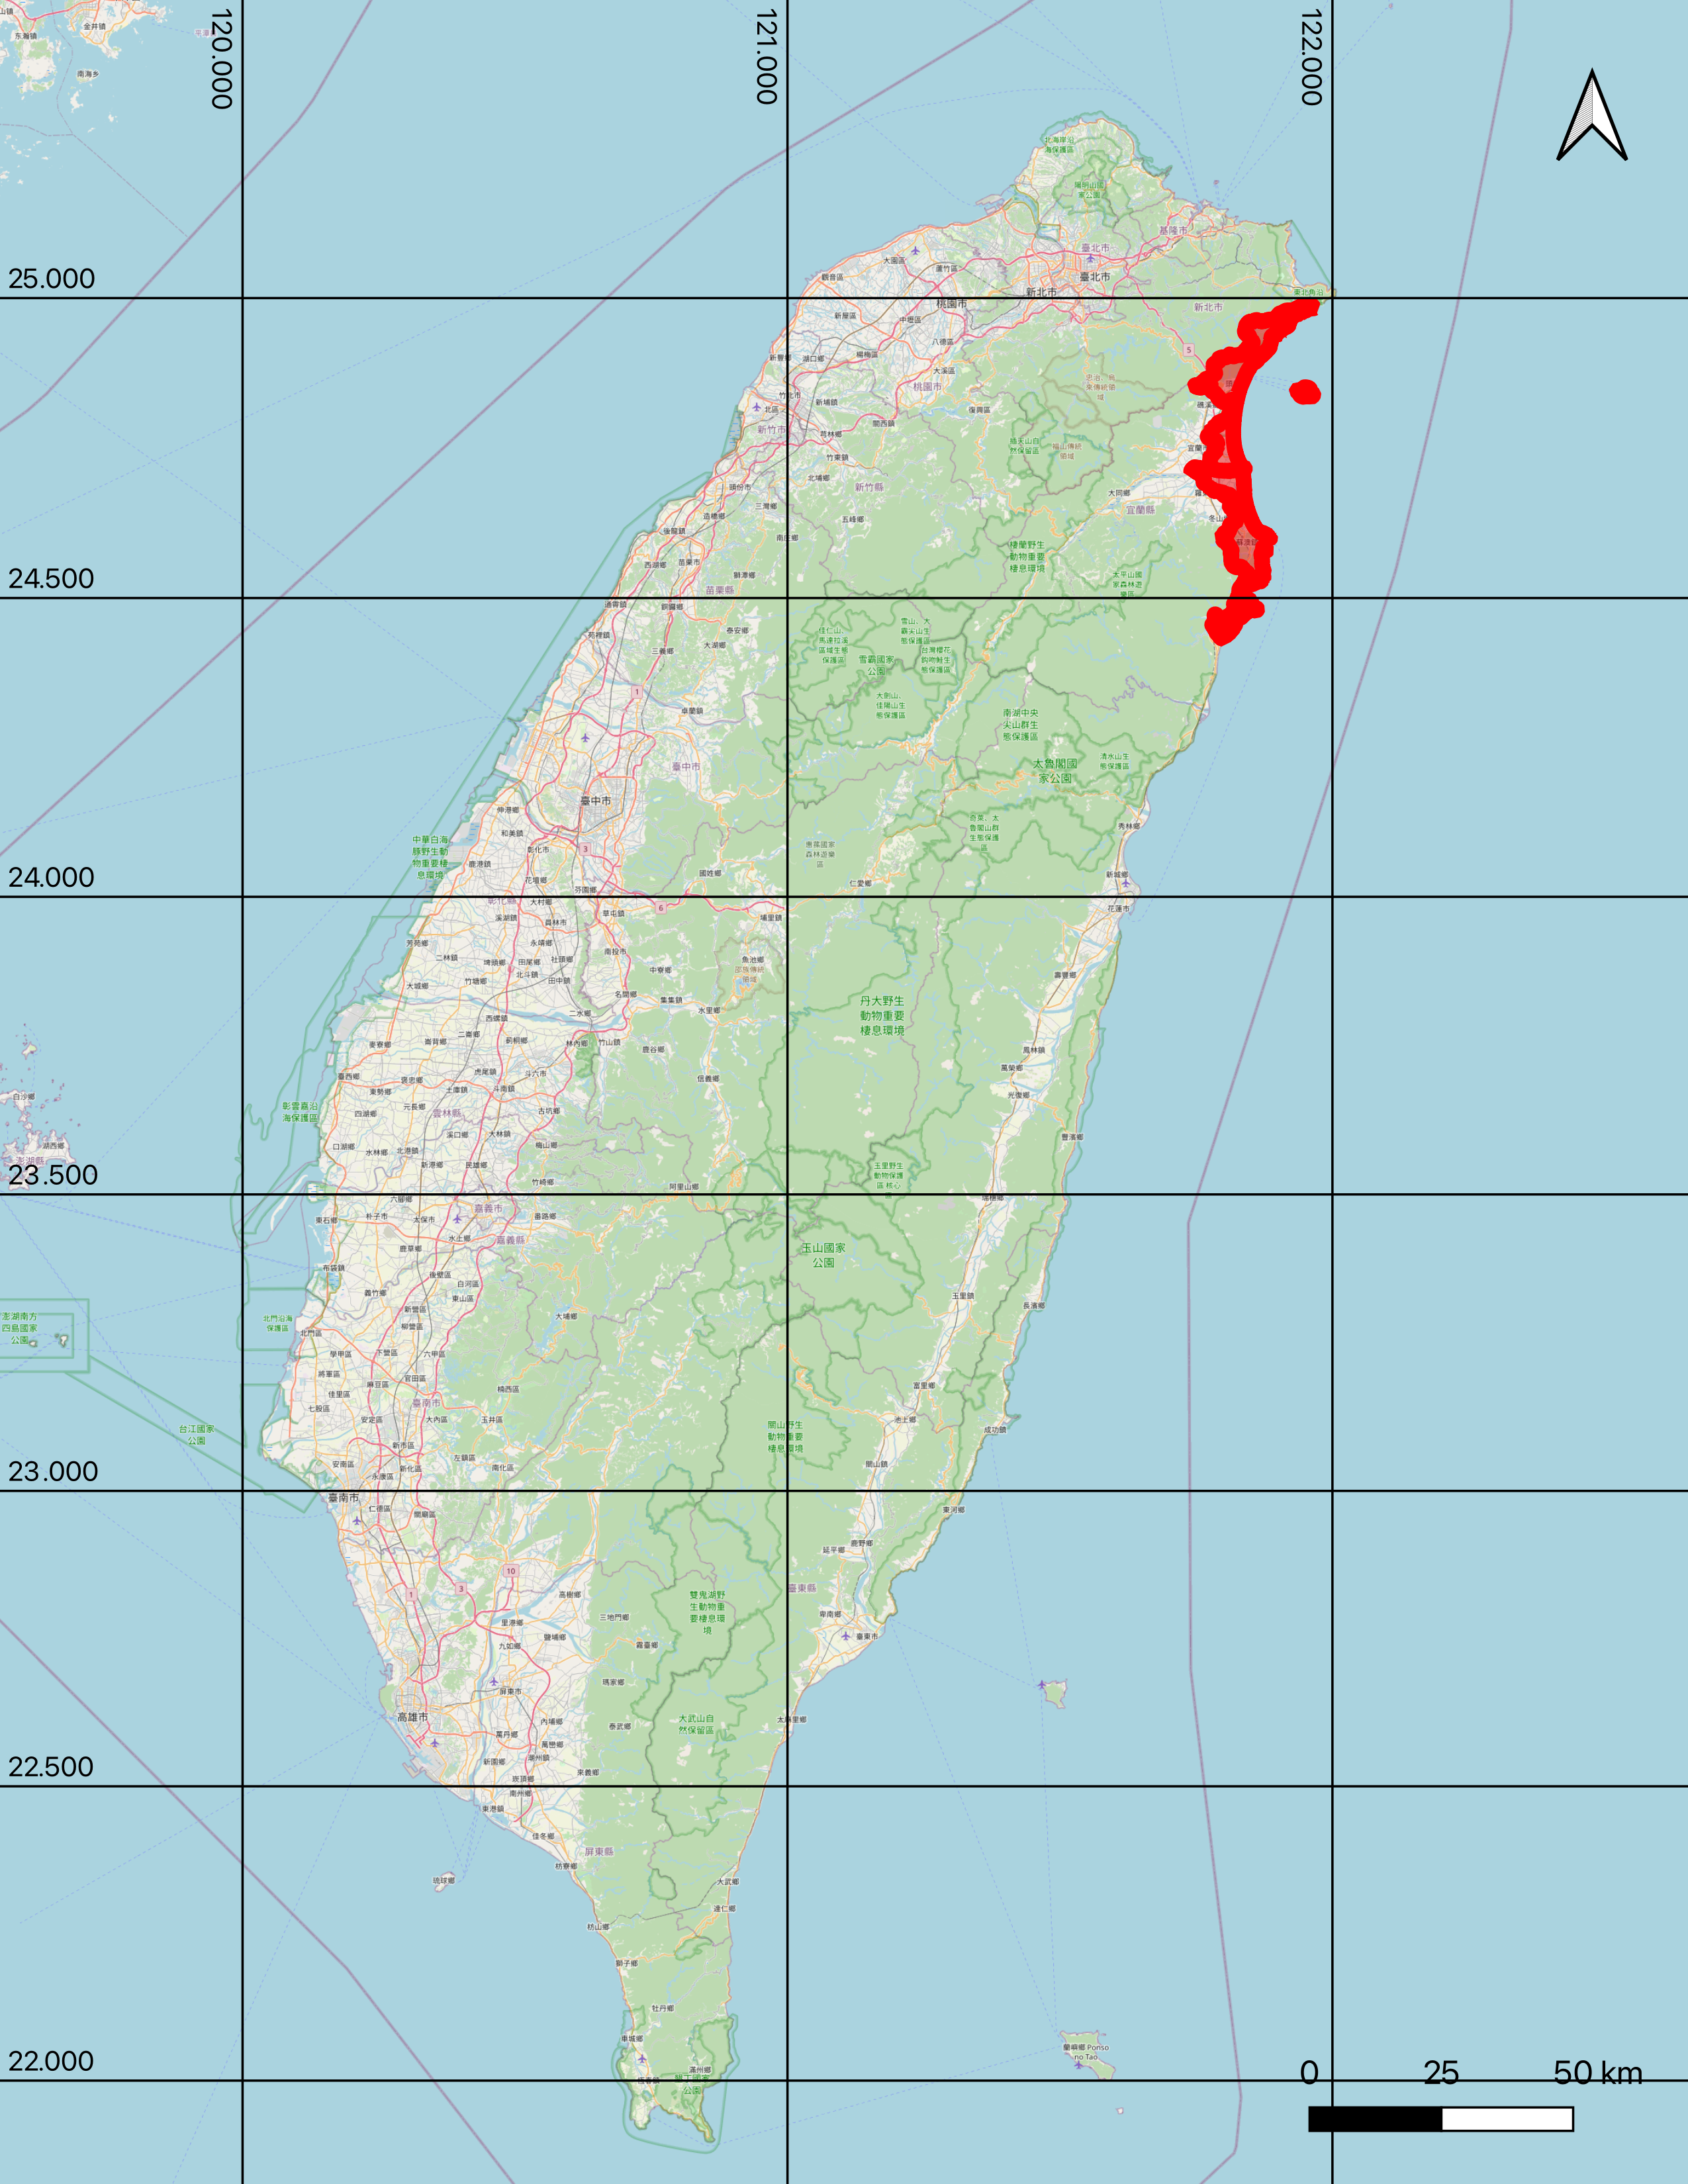
\includegraphics[width=0.95\linewidth]{figures/cases/case5_1.png} & 在台灣東北部沿岸 & 東北沿海地區 & 東北部沿海地區，包含宜蘭縣沿海及鄰近釣魚台海域，靠近蘇澳港及龜山島，並延伸至琉球群島北部海域。 \\ \hline
5-2 &
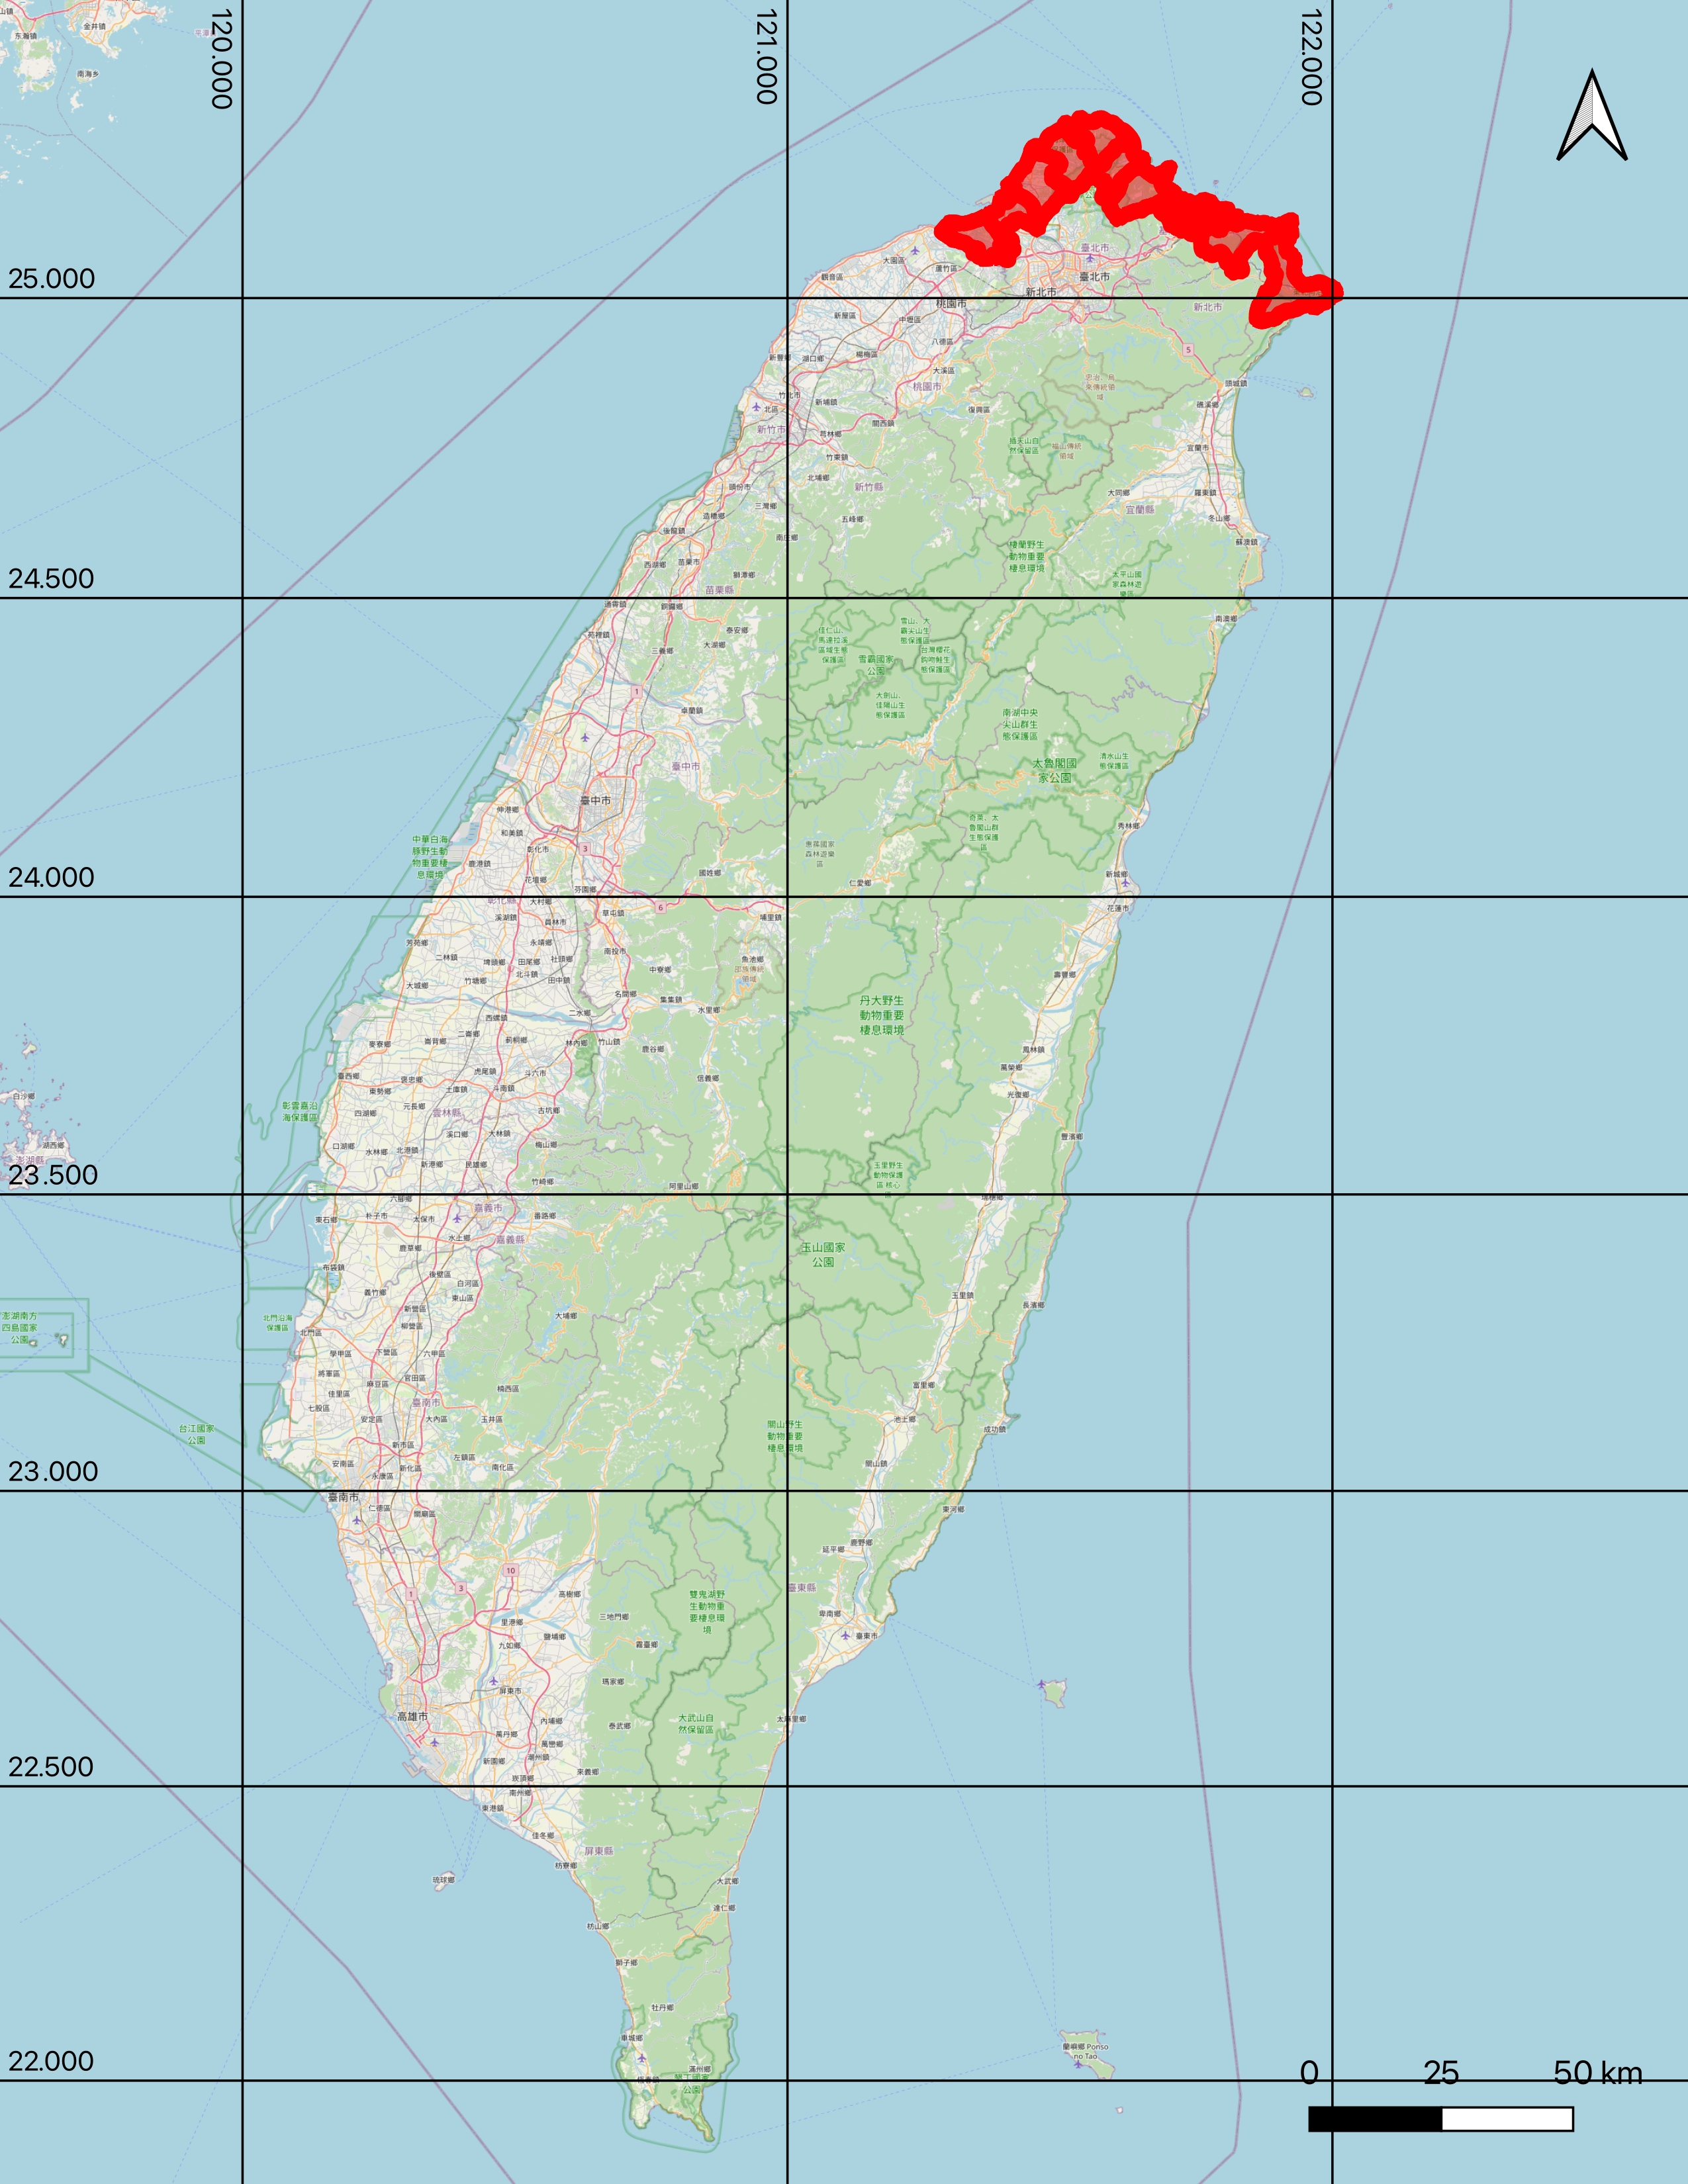
\includegraphics[width=0.95\linewidth]{figures/cases/case5_2.png} & 基隆市外海* & 北部沿海地區 & 位於台北市東北部沿海地區，鄰近基隆市，靠近基隆河口，涵蓋新北市瑞芳區及貢寮區部分地區，延伸至東北角海岸國家風景區，包含福隆海水浴場及鼻頭角等地標，並接近台2線沿海公路。 \\ \hline
5-3 &
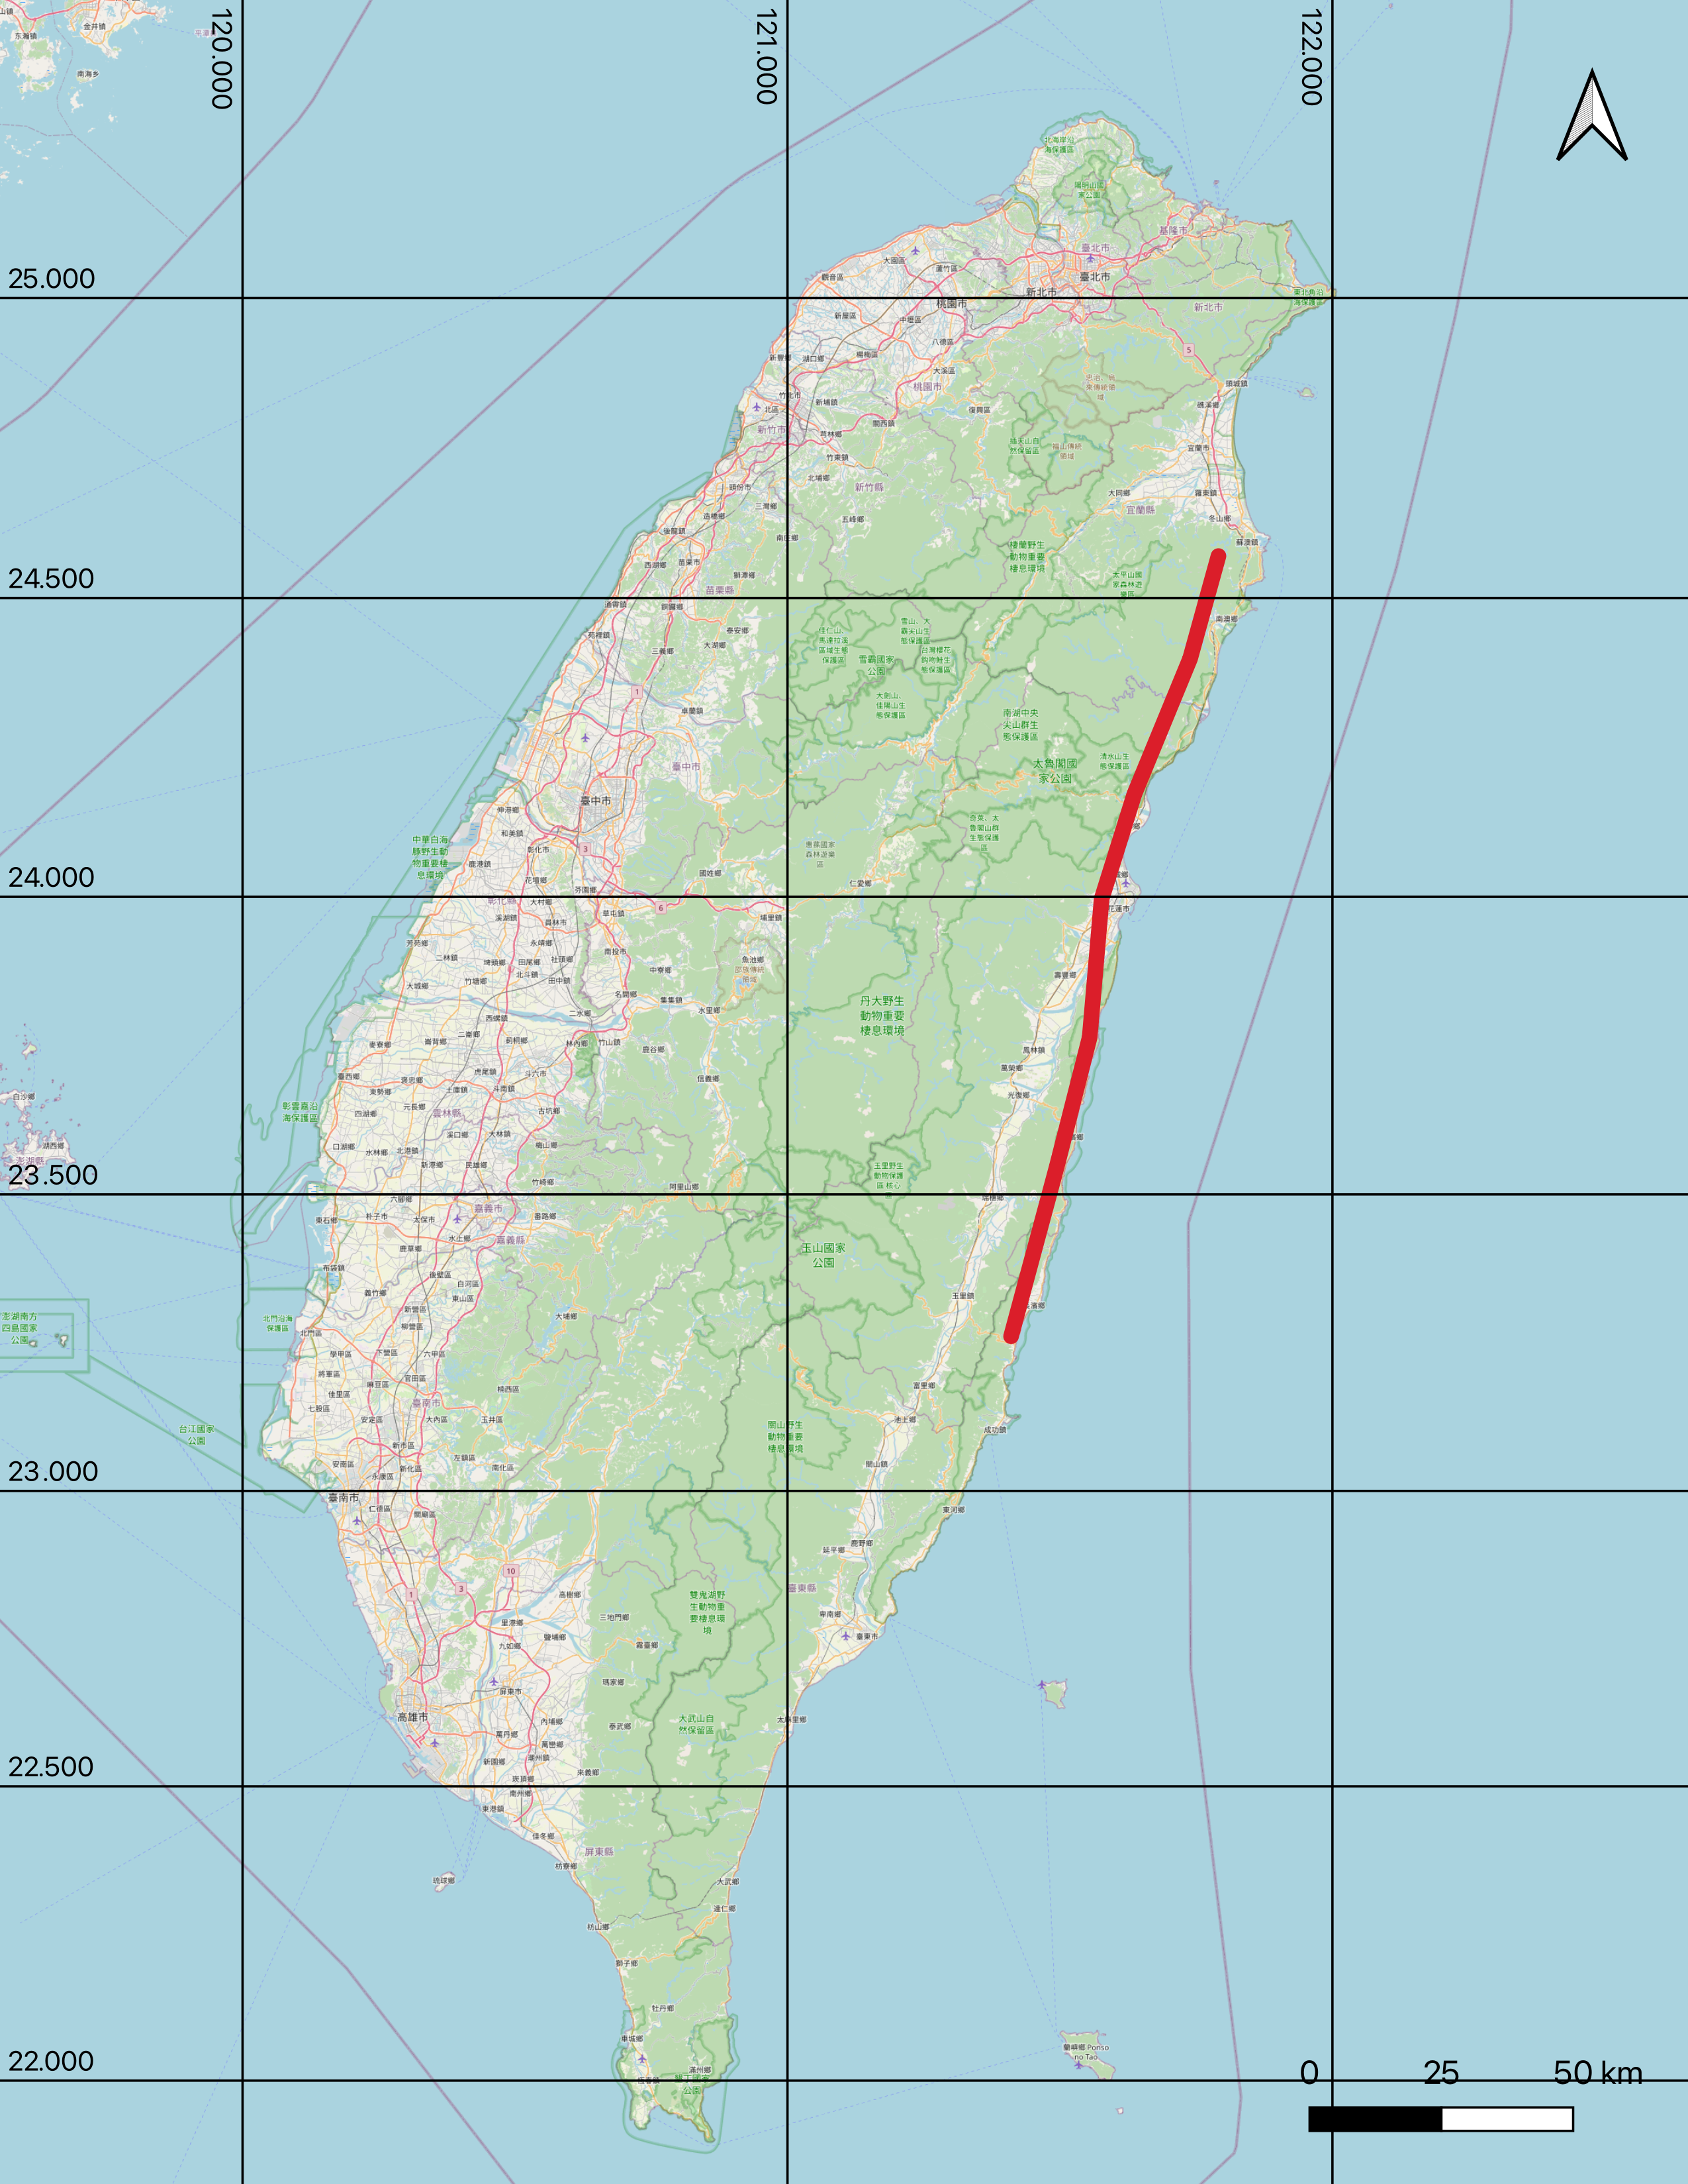
\includegraphics[width=0.95\linewidth]{figures/cases/case5_3.png} & 在台灣東部沿岸 & 東部沿海地區 & 位於台北市東北部沿海地區，鄰近基隆市，靠近淡水河岸，並延伸至新北市瑞芳區，涵蓋基隆港及周邊商業區。\\
5-4 & & & 海峽沿海地區 & \\ \hline
5-5 & & & 西南沿海地區 & \\ \hline
5-5 & & & 東南沿海地區 & \\
\end{longtable}
}

\clearpage
\section{評估}

\begin{table}[htbp]
\centering
\caption{標記之真值}
\label{tab:groundTrue}
\begin{adjustbox}{max width=\textwidth}
\renewcommand{\arraystretch}{1.4}
\begin{tabular}{>{\centering\arraybackslash}m{1cm} >{\centering\arraybackslash}m{16cm} }
\toprule
項次 & 內容 \\
\toprule
1-1 & ("在", "新北市", None), (None, "瑞芳區", None), (None, "萬瑞快速道路", "上"), ("西行", None, None), (None, "瑞濱端", None), (None, "龍潭堵隧道", "內") \\
\hline
1-2 & (None, None, "北上"), ("在", "中山高速公路", "上"), (None, "10.5公里", "處"), (None, "汐止交流道", None) \\
\hline
1-3 & ("在", "臺北市",  None), (None, "大安區", None), (None, "和平東路二段118巷2弄", None), (None, "科技大樓", "後方"), (None, "科技部", "附近") \\
\hline
1-4 & ("在", "臺北市",  None), (None, "大同區", None), (None, "民權西路", "路口"), (None, "承德路二段", "路口"), (None, "捷運民權西路站", "附近"), (None, "台灣銀行", "附近"), (None, "台北大橋", "前") \\
\hline
1-5 & ("在", "臺北市",  None), (None, "大安區", None), (None, "建國南北快速道路", None), (None, "忠孝東路三段", "上方"), ("鄰近", "臺北科技大學", None) \\
\hline
1-6 & (None, "台北大橋",  None), ("往", "台北", None), ("在", "新店溪", "上") \\
\hline
2-1 & (None, "新店溪", None), (None, "新店溪", "沿岸"), (None, "翡翠水庫", "下游")\\
\hline
2-2 & (None, "大漢溪", None), (None, "淡水河", None), (None, "新店溪", "沿岸"), (None, "淡水河", "沿岸"), (None, "石門水庫", "下游")\\
\hline
2-3 &  (None, "木瓜溪", "下游"), (None, "木瓜溪", "沿岸") \\
\hline
3-1 & (None, "台灣", "東北部") \\
\hline
3-2 & (None, "台灣", "東北部"),  (None, "花蓮", "地區") \\
\hline
3-3 & (None, "台灣", "東北部"),  (None, "宜花", "地區") \\
\hline
4-1 & (None, "烏來區", None), (None, "石碇區", None), (None, "南勢溪", "上游"), (None, "崩山溪", "上游")\\
\hline
4-2 & (None, "基隆市", "山區"), (None, "五分山", None)\\
\hline
4-3 & (None, "七堵區", None), (None, "暖暖區", None), (None, "八堵區", None)\\
\hline
5-1 &  (None, "東北部", "沿海"), (None, "宜蘭縣", "沿海")\\
\hline
5-2 &  (None, "北部", "沿海") \\
\hline
5-3 & (None, "東部", "沿海"), (None, "宜花東", "沿海") \\
\bottomrule
\end{tabular}
\end{adjustbox}
\end{table}

\clearpage
\section{GPT-4o Prompt}
 
你的任務是執行逆向地理編碼，並針對傳入的geojson，產生對應的文字式位置描述。
請依據以下格式：
ＯＯ（依照情境，例如：交通）描述：針對目標物件本身或者鄰近地標或參考物的相對位置（如：ＯＯ（依照情境，例如：「國道一號南下」））。
同時，生成的描述參考（但不一定要放入你最終的位置描述上）下列：
  \begin{enumerate}
    \item 絕對位置名稱，例如城市名稱或特定地點名稱。
    \item 鄰近的地標或參考物，描述其相對於目標物件的位置。
    \item 靠近目標物件的主要道路和交叉路口。
    \item 附近的自然地理特徵。
    \item 提供更清晰位置的行政區劃。
    \item 該區域的環境特徵或土地使用情況。
  \end{enumerate}
請根據以上要求生成一個 2 到 50 字以內綜合多筆圖徵產出「一個」綜合式位置描述段落。